\chapter{Анализ методов и средств поддержки исследований с интенсивным использованием данных} \label{chapt1}

\section{Гипотезы, теории и законы: историческая перспектива} \label{sect1_1}

В настоящее время исследования с интенсивным использованием данных (ИИИД) развиваются в соответствии с Четвертой 
парадигмой \cite{Hey2009} научных изысканий, последовавшей за тремя исторически предшествовавшими ей парадигмами 
развития науки. Это подчеркивает, что наука в целом все более полагается на данные, которые и являются ключевым 
источником научного открытия. Появление Четвертой парадигмы обусловлено чрезвычайно большими объемами данных, 
получаемых от приборов, датчиков, моделей, а также в результате накопления данных в Интернете и социальных сетях. 
Фундаментальная цель ИИИД "--- получение (вывод) знаний на основе совокупных данных, организованных в сетевые 
инфраструктуры. Открытый доступ к большим объемам данных становится, таким образом, ключевой предпосылкой к открытиям 
XXI века. Исследования с интенсивным использованием данных находятся на пересечении методов ИИИД-ИТ и направлены 
на создание эффективных технологий анализа данных в ИИИД, охватывающих научные и другие информационноёмкие сферы 
(включая финансы, экономику, социальную среду, бизнес и др.).

\nomenclature{ИИИД}{исследования с интенсивным использованием данных}
\nomenclature{ИТ}{информационные технологии}


Наука ставит своей целью дать осмысленное описание мира природных явлений, используя то, что известно как его законы, 
гипотезы и теории. Гипотезы, теории и законы, по существу своему, имеют одинаково фундаментальный 
характер~(\cref{fig:hypothesis_repr}) \cite{McComas2005}. 

\begin{figure}[ht]
    \centering
    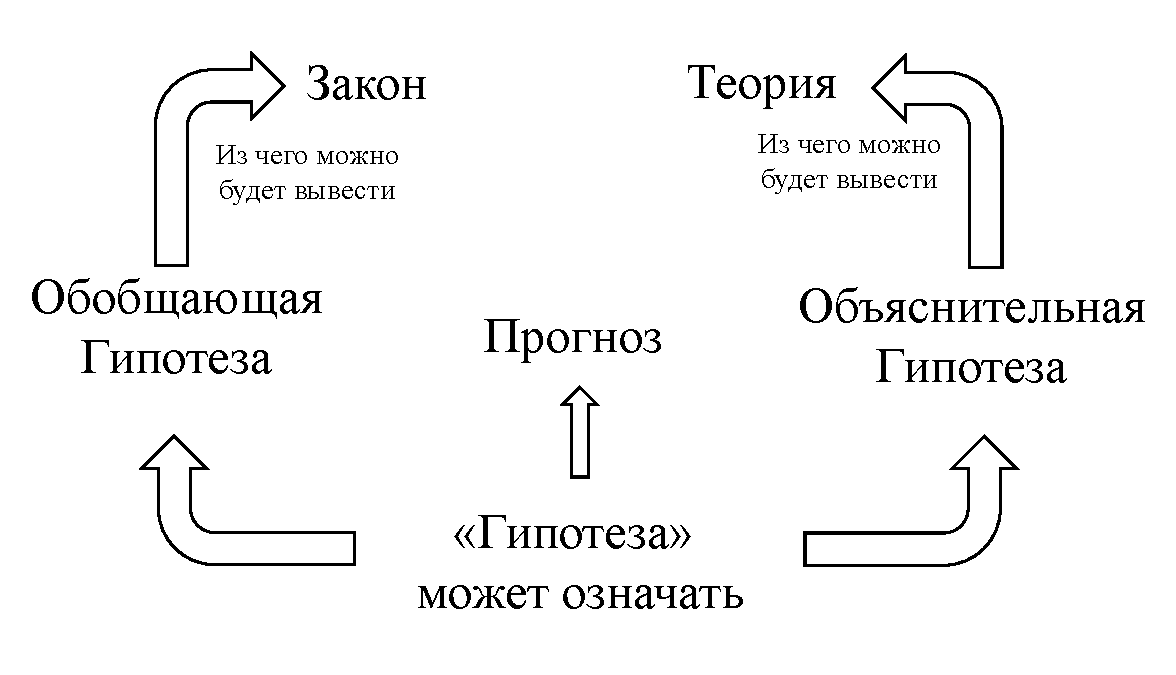
\includegraphics[width=0.7\linewidth]{images/hypothesis_life.pdf}
    \caption{Воплощение гипотезы.}\label{fig:hypothesis_repr}
\end{figure}

\textit{Научная гипотеза} есть предлагаемое объяснение явления, которое еще должно быть подвергнуто строгой проверке. 
В отличие от этого, \textit{научная теория} уже прошла всесторонние испытания и широко принята в качестве точного 
объяснения, стоящего за наблюдением. \textit{Научный закон} - это утверждение, которое показывает некоторую 
упорядоченность или регулярность в природе, \textit{существование неизменной связи между определенным комплексом 
условий и определенными явлениями}. В точных науках законы, как правило, выражаются в виде математических зависимостей. 
Гипотезы лежат в основе законов, а тщательно проверенные, подтвержденные гипотезы становятся теориями. В то же время 
законы не перестают быть законами, если они изначально не появились как гипотезы и не прошли стадию существования 
в качестве теорий.

Несмотря на то, что теории и законы являются разными видами знания, они все же представляют собой лишь разные формы 
одного и того же конструкта знания. Законы представляют собой обобщения, принципы или паттерны в природе, а теории 
разъясняют такие обобщения. Необходимо отметить, что классификация, представленная на ~\cref{fig:hypothesis_repr}, 
субъективна. Работа \cite{Rao1998} приводит примеры, показывающие, что различия между законами, гипотезами и теориями 
заключаются лишь в том, что они находятся на разных уровнях приемлемости "--- в зависимости от количества накопленных 
эмпирических доказательств. Таким образом, нет существенного различия между конструктами, которые используются для 
выражения гипотез, теорий и законов. 

Едва ли можно переоценить важность роли гипотез в научных исследованиях. В издании книги А. Пуанкаре\cite{Poincare2015} 
подчеркнуто, что \textit{наука не существует без гипотез}. Поэтому неудивительно, что в научных исследованиях и 
соответствующих публикациях столь много внимания посвящено методам оперирования гипотезами с применением методов 
информатики в процессе экспериментального изучения и моделирования различных явлений. Мысль о том, что наукам, 
интенсивно использующим данные, и тем, которые опираются на гипотезы, необходимы новые подходы, пронизывает всю эту 
работу. Симбиоз такого рода, вместе с традицией науки, движимой гипотезами (<<сначала гипотеза, потом эксперимент>>), 
может привести также и к широкому применению другого метода исследований: <<сначала эксперимент, потом гипотеза>>. 
Во многих случаях порядок <<сначала эксперимент>> в ИИИД мотивируется необходимостью анализа существующих массивов 
данных с целью создания гипотезы. На \cref{fig:knowledge_production} показаны именно такие пути производства 
знаний~\cite{McComas2005}. <<Обобщение>> здесь означает любое подмножество гипотез, теорий и законов, 
а <<свидетельство>> "--- это любое подмножество всех фактов, накопленных в рамках конкретного ИИИД.

\begin{figure}[ht]
    \centering
    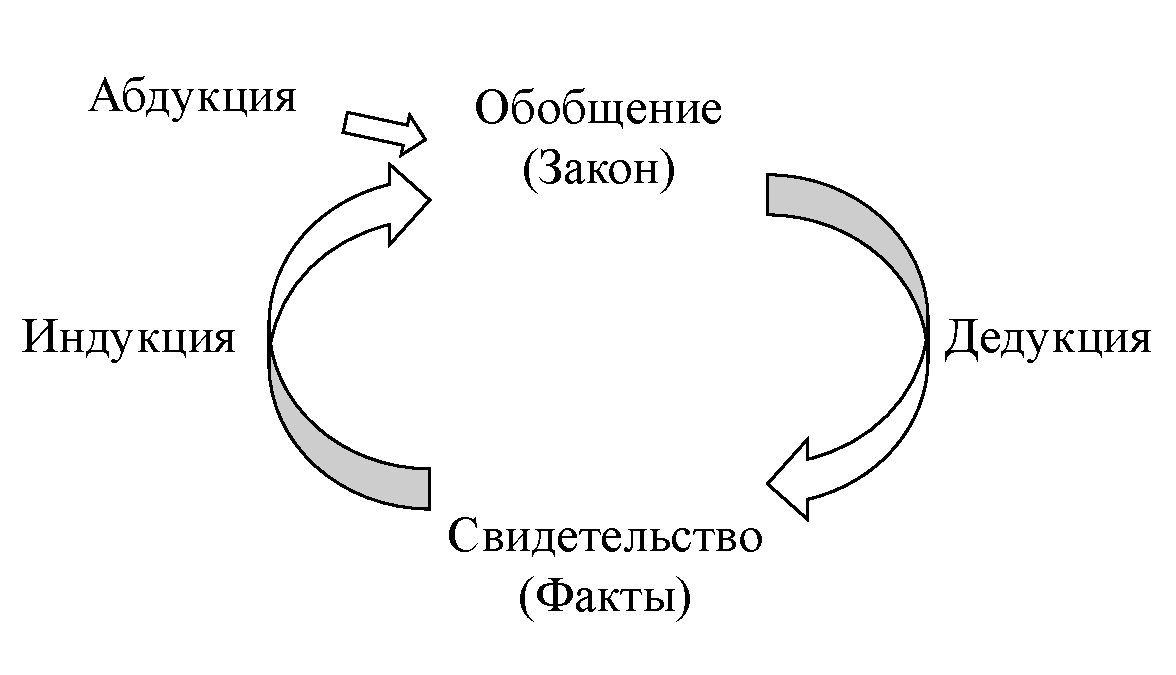
\includegraphics[width=0.7\linewidth]{images/science_lifecycle}
    \caption{Развернутая диаграмма производства знаний.}\label{fig:knowledge_production}
\end{figure}

Каждый исследователь занимается сбором и интерпретацией эмпирических доказательств, а сам процесс называется индукцией. 
Это "--- методика, в которой собираются и рассматриваются разрозненные элементы доказательства до того момента, когда 
открывается закон или изобретается теория. Первым формализовал понятие индукции Ф.~Бэкон \cite{Bacon2000}. 
Предложенный им метод (наивной) индукции (\cref{fig:knowledge_production}) традиционно является основополагающим 
методом, с помощью которого человек, как правило, делал обобщения, позволяющие предсказывать события. Затруднения, 
связанные с индукцией, заключаются в том, что невозможно собрать воедино все наблюдения, касающиеся данного явления 
в любое время "--- в прошлом, настоящем и будущем.  

\textit{Закон} обобщает массу наблюдений. В целом, закон представляет собой группу связанных между собой неоспоримых 
гипотез, использующих небольшое количество фундаментальных понятий и уравнений, определяющих поведение некоторого 
множества явлений. Закон не является попыткой объяснить, <<почему так происходит>>, он просто констатирует факт. 
Формулирование нового закона начинается с индукции, когда факты наслаиваются на другие релевантные факты. В целях 
проверки справедливости закона полезна дедукция.  На \cref{fig:knowledge_production} показано, что действительно 
справедливый закон всегда позволяет точное предсказание еще неизвестных фактов.  Кроме того, существует абдукция 
\cite{Menzies1996}, процесс проверки данной гипотезы путем последовательно аппроксимирующего логического рассуждения. 
Согласно этому принципу, всякое рассуждение справедливо, если оно является наилучшим объяснением данного множества 
известных данных. Абдуктивная валидация является общепринятой практикой формирования научных гипотез.

В \cite{Poincare2015} рассматриваются два рода используемых в науке гипотез: 

\begin{enumerate}
    \item Гипотезы, которые ценны именно потому, что они могут быть подтверждены или, напротив, опровергнуты путем 
        прямого обращения к тому, что предлагает опыт.
    \item Гипотезы, которые, несмотря на то, что опыт предполагает их, являются ценными, невзирая на то, или даже 
        вследствие того, что опыт не может ни подтвердить их, ни опровергнуть.
\end{enumerate}

Особенности науки, обуславливаемые использованием гипотез второго рода, рассматриваются А. Пуанкаре как <<представляющий 
собой присущий человеку способ рассмотрения природы, интерпретацию, а не описание или предсказание объективных 
природных фактов, приспособление наших концепций внутренним потребностям нашего разума>>. По мнению А.~Пуанкаре, 
центральной проблемой научной логики является проблема соотношения между двумя фундаментально разными видами гипотез, 
а именно между теми, которые не могут быть подтверждены или опровергнуты опытным путем, и теми, которые могут 
быть эмпирически проверены.

Любая полезная гипотеза позволяет прогнозирование посредством рассуждений (включая дедуктивные рассуждения). 
Она может предсказать исход эксперимента в лабораторных условиях или наблюдение природного явления. К прогнозированию 
также может привлекаться статистика при допущении, что гипотеза может быть 
фальсифицируемой (опровергаемой) \cite{Popper2005}, и что нельзя рассматривать предположение или теорию в качестве 
научных, если они не допускают самой возможности их несправедливости. Можно провести границу между гипотезами, если 
называть научными только те из них, для которых можно указать (заранее) одно или несколько потенциально 
опровергающих доказательств "--- таких, как соответствующие эксперименты. 
Опровержение предполагается дедуктивным, но не индуктивным.

Другие философы науки отвергают критерий фальсифицируемости или дополняли его другими критериями "--- 
например, критерием проверяемости (познавательно значимыми являются только такие утверждения 
относительно нашего мира, которые подтверждаются эмпирически или логически необходимы). 
Они утверждают, что наука движется в процессе <<индукции>> "--- т.е. путем поиска подтверждений предположениям 
(гипотезам). К.~Поппер считал, что подтверждения 
никогда не являются твердыми. Опровержение, однако, может оказаться неожиданным и определенным \cite{Popper2005}. 
А.~Эйнштейн высказался следующим образом: <<Никакое количество экспериментов никогда не сможет доказать, что я прав; 
однако один-единственный эксперимент сможет доказать, что я не прав>>. Для ученых и философов, не придерживающихся 
мнения К.~Поппера, наука работает, в основном, на базе индукции (подтверждения), а также, хотя и реже, на базе 
неподтверждения (опровержения). Языком науки почти всегда является язык индукции. В рамках данного обзора приемлемы 
оба философских подхода к гипотезам. Иногда такой способ рассуждения называется 
\textit{гипотетико-дедуктивным методом}. В соответствии с этим методом научное исследование выполняется путем 
формулирования гипотезы в некоторой форме, которая предположительно могла бы быть опровергнута проверкой с помощью 
наблюдаемых данных. Проверка, которая могла бы противоречить и реально противоречит прогнозам гипотезы, признается 
опровержением гипотезы. Проверка, которая могла бы противоречить, но реально не противоречит прогнозам гипотезы, 
подтверждает данную теорию.

Научный метод включает в себя эксперимент, необходимый для проверки, может ли гипотеза дать адекватный ответ на 
поставленный вопрос. Прогноз на основе гипотезы предполагает проверку (наблюдение или эксперимент) гипотезы, которая 
таким образом и становится проверяемой. Если гипотеза не порождает возможность наблюдательной проверки, исследователь 
никак не может её использовать.

Например, можно выдвинуть непроверяемую гипотезу <<Наша вселенная погружена в другую, более масштабную вселенную, с 
которой мы не можем иметь абсолютно никакого контакта>>; вот потенциально подтверждаемая (хотя и потенциально 
проверяемая) гипотеза: <<Во вселенной есть другие обитаемые планеты>>; а вот научная гипотеза (проверяемая и 
подтверждаемая): <<Любые два предмета, сброшенные (одновременно) с одной и той же высоты над поверхностью земли, 
упадут на эту поверхность в один и тот же момент времени, если нет сопротивления воздуха>> \cite{Stanbrough2022}.

\textit{Задачу (научный вопрос)} следует формулировать в форме <<какое соотношение существует между двумя и 
более переменными>>. Постановка задачи должна быть такой, которая подразумевает возможности эмпирической 
проверки "--- в противном случае задача не будет научной. Задачи и гипотезы, будучи обобщенными формулировками 
соотношений, дают возможность делать вывод о конкретных эмпирических явлениях, подразумеваемых задачами и гипотезами. 
В такого рода процессе гипотезы могут быть выдвинуты на основе теории или других гипотез. Задача не может быть научно 
разрешена, если она не сведена к виду гипотезы, поскольку задача не может быть проверена 
непосредственно \cite{Azorin1966}.

Большинство формальных гипотез объединяют концепции, указывая на ожидаемые соотношения между \textit{предположениями}. 
Когда множество гипотез образует группу, они становятся \textit{концептуальной структурой}. Если концептуальная 
структура является комплексной и включает в себя каузальность или объяснение, её обычно называют 
\textit{теорией} \cite{Hempel1952}. Вообще говоря, гипотезы должны отражать многовариантную сложность реальности. 
\textit{Научная теория} обобщает гипотезу или группу гипотез, поддержанных неоднократными проверками. Теория 
справедлива, если нет ни одного противоречащего ей факта. \textit{Научная парадигма} объясняет рабочее множество 
теорий, на которых основана наука.

\section{Роль гипотез и моделей в исследованиях с интенсивным 
         использованием данных: фундаментальные принципы}\label{sect1_2}

\subsection{Различные представления научных гипотез}\label{sect1_2_1}
Существует множество представлений научных гипотез в исследованиях 
с интенсивным использованием данных (см. \cref{fig:hypothesis_representation}).

\begin{figure}[ht]
    \centering
    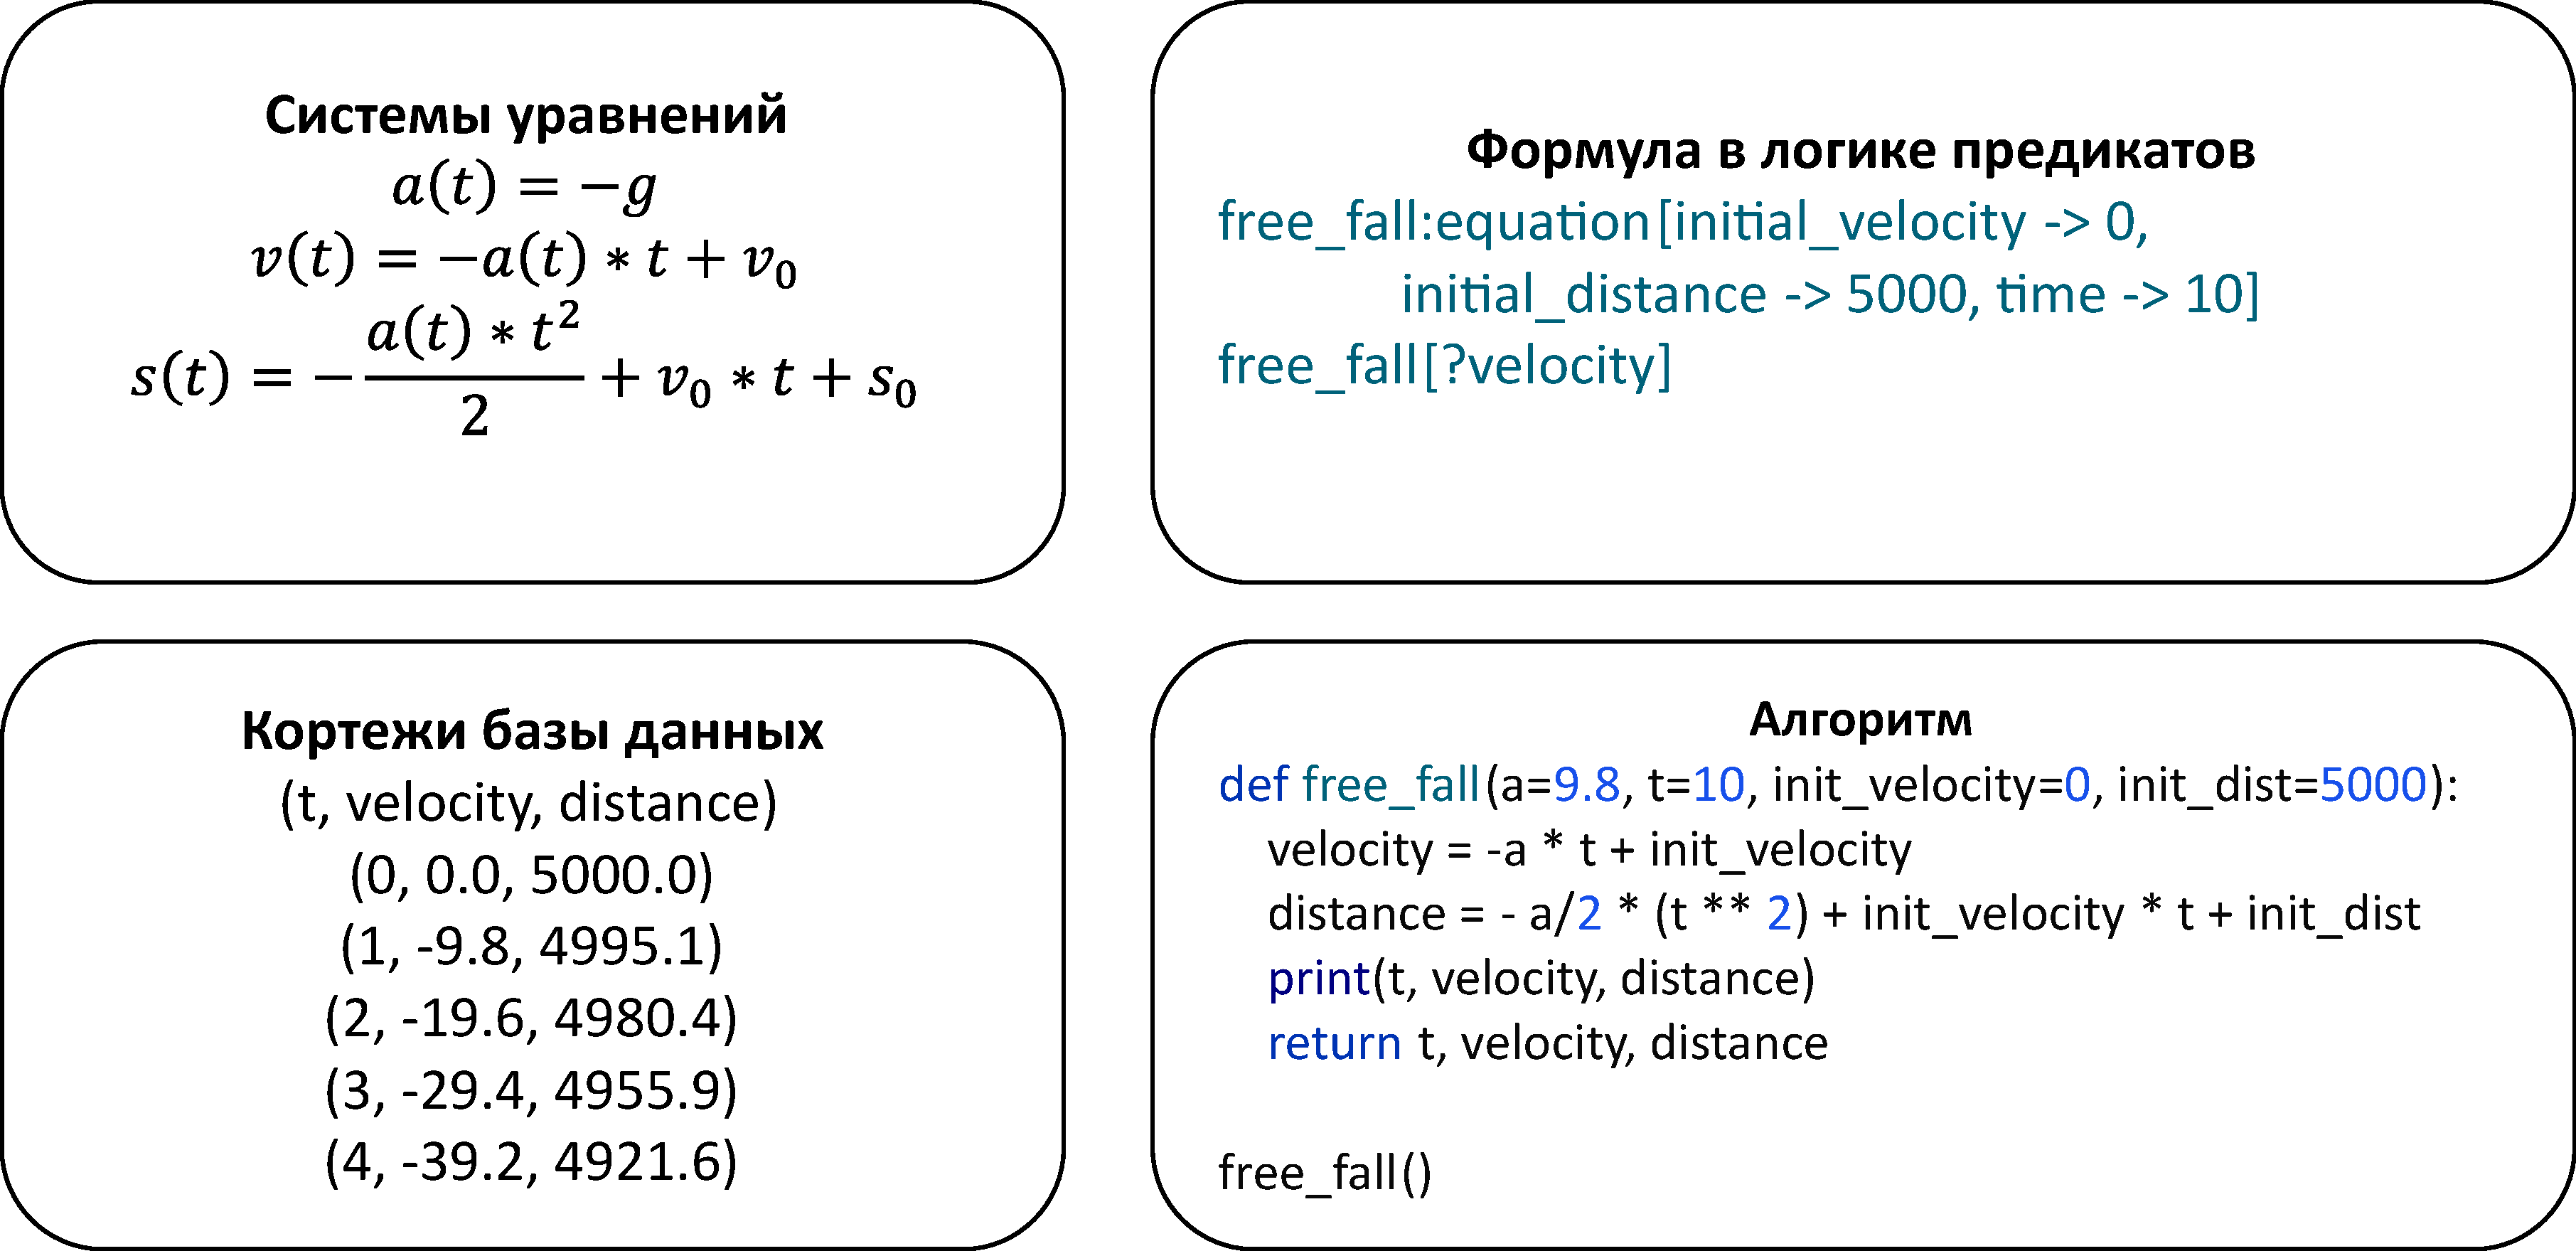
\includegraphics[width=1.0\linewidth]{images/hypothesis_representation.pdf}
    \caption{Различные представления научных гипотез.}\label{fig:hypothesis_representation}
\end{figure}

Например, научные гипотезы имеют вид математической модели. Иногда их также можно формулировать как предложения в 
логике предикатов, констатирующие, что в определенном случае рассматриваемое явление обладает некоторой 
характеристикой, а также каузальные утверждения, имеющие общую форму универсальных утверждений, 
констатирующих, что явление во всех случаях имеет определенную характеристику (напр., для всех x, если 
x "--- лебедь, то x "--- белый). Научная гипотеза, рассматриваемая как декларативное утверждение, указывает 
прогнозируемое соотношение (ассоциативное или каузальное) между двумя или более переменными (зависимыми или 
независимыми и зависимыми). В случае каузального соотношения изменение, имеющее своей причиной независимую переменную, 
прогнозируется зависимой переменной. Переменные чаще всего связаны некаузально (ассоциативно) \cite{Haber2009}.

В экспериментальных работах исследователь манипулирует независимой переменной. Зависимую переменную часто считают 
следствием или предполагаемым результатом, который изменяется вслед за изменением независимой переменной. Зависимой 
переменной не манипулируют. Она наблюдается и принимается в качестве изменяющейся с изменением независимой переменной. 
Прогнозирование делается в направлении от независимой переменной к зависимой переменной. Исследователя интересует 
понимание, объяснение или прогнозирование именно зависимой переменной \cite{Haber2009}.

В том случае, когда исследуется возможная корреляция или подобное соотношение между переменными (как, например, 
является ли предлагаемый препарат эффективным в лечении болезни, т.е., по крайней мере, до некоторой степени и для 
некоторых пациентов), немногочисленные случаи, где испытываемое лекарство не дает результата, не опровергают гипотезу. 
На самом деле, для определения того, насколько вероятно, что общий эффект будет наблюдаться, если не существует 
реального соотношения, заложенного в гипотезе, используются статистические испытания. Если такая вероятность достаточно 
мала, существование некоторого соотношения может быть допущено. При статистическом испытании гипотез сравниваются две 
гипотезы, называемые нулевой гипотезой и альтернативной гипотезой. Нулевая гипотеза утверждает, что нет соотношения 
между исследуемыми явлениями (переменными), или, по крайней мере, его нет в форме, предлагаемой альтернативной 
гипотезы. Альтернативная гипотеза, как и предполагает её наименование, это альтернатива нулевой гипотезы: она содержит 
утверждение, что некоторое соотношение существует.

Альтернативные гипотезы, как правило, используются чаще, чем нулевые, поскольку они более желательны для реализации 
ожиданий исследователя. Однако в любом исследовании, использующем статистический анализ, как правило, всё же 
допускается лежащая в основе нулевая гипотеза \cite{Haber2009}. Здесь важно то, что положение <<не отвергайте нулевую 
гипотезу>> необязательно означает, что нулевая гипотеза справедлива. Оно лишь предполагает, что нет существенных 
доказательств в пользу альтернативной гипотезы в противовес нулевой гипотезы. Отбрасывание же нулевой гипотезы 
предполагает, что альтернативная гипотеза может оказаться справедливой.

Элементы движимых гипотезами исследований и их соотношения показаны на \cref{fig:hypothesis_real} 
\cite{Goncalves2013, Porto2011}. Соотношения треугольника гипотезы (\textit{объясняет, формулирует, представляет}) 
конструктивны для принятия исследователем окончательного решения: выбрать конкретную модель $m_i$ с целью 
формулирования гипотезы $h_i$, которая предназначена для объяснения явления $p_i$. 

\begin{figure}[ht]
    \centering
    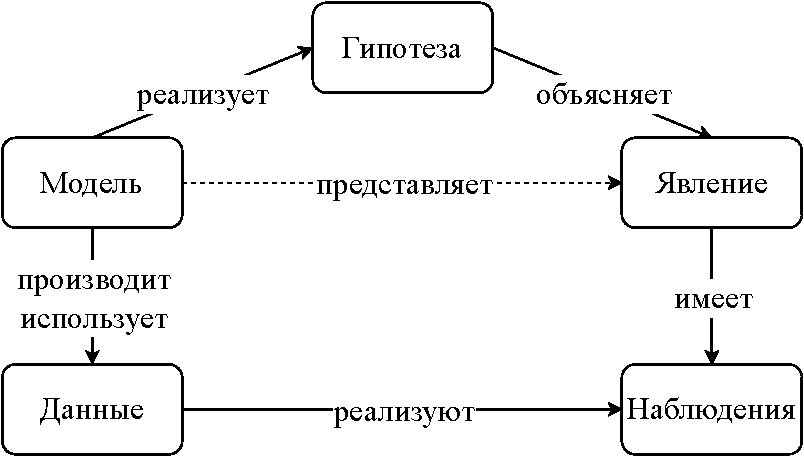
\includegraphics[width=0.7\linewidth]{images/hypothesis_real}
    \caption{Элементы движимых гипотезами исследований.}\label{fig:hypothesis_real}
\end{figure}

В работе \cite{Goncalves2013} предлагается решетчатая структура соединения гипотез, как показано на 
\cref{fig:hypothesis_relation}. Решетка гипотез образуется при рассмотрении множества гипотез, расположенных 
в строгом порядке \textit{derived\textunderscore by} "--- была выведена из (снизу вверх). Гипотезы, 
непосредственно выведенные из одной единственной гипотезы, называются атомарными, в то время как те, которые выведены, 
по крайней мере, из двух гипотез, называются комплексными.

\begin{figure}[ht]
    \centering
    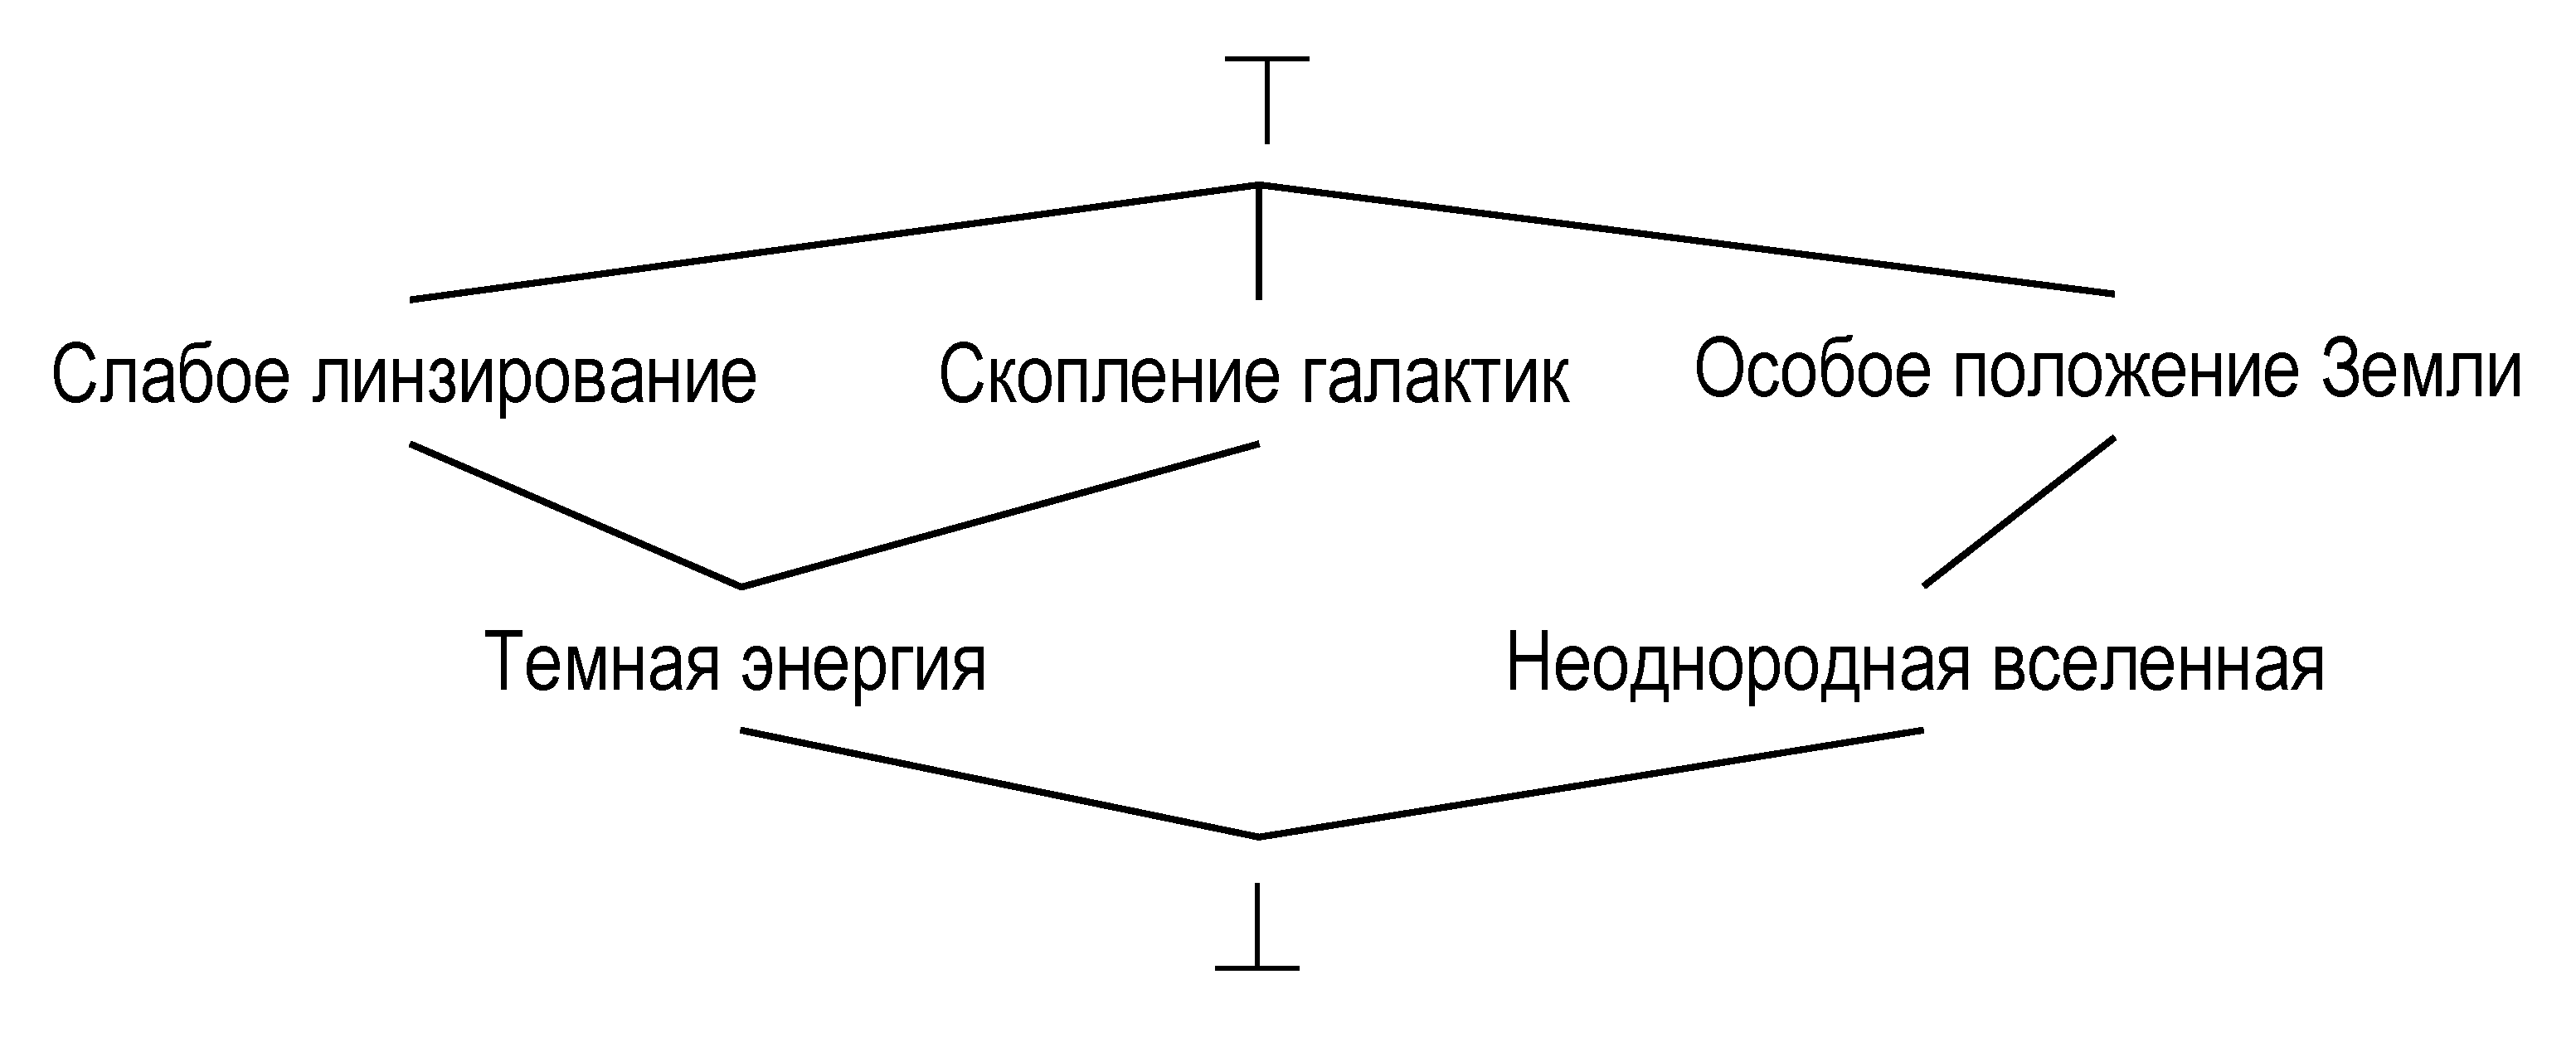
\includegraphics[width=0.7\linewidth]{images/hypothesis_relation.pdf}
    \caption{Теоретическое представление отношений в решетке гипотез.}\label{fig:hypothesis_relation}
\end{figure}

Решетка гипотез разворачивается в модель и изоморфные решетки явлений в соответствии с треугольником 
гипотез \cref{fig:hypothesis_real}. Решетки изоморфны, если исследователь выбирает такие подмножества $M$ (моделей), 
$H$ (гипотез) и $P$ (явление) так, что они формулируют, объясняют и представляют как один в один, так и отображения 
на себя (т.е. взаимно-однозначные соответствия), рассматриваемые как отображения, сохраняющие структуру (морфизмы). 
Пример изоморфной решетки показан на \cref{fig:lattice_fluid}. Эта решетка соответствует случаю в вычислительной 
гемодинамике, рассмотренному в \cite{Goncalves2013}. Здесь модель $m_1$ формулирует гипотезу $h_1$, которая объясняет 
явление $p_1$. Подобным же образом модель $m_2$ формулирует $h_2$, которая объясняет $p_2$, и т.д. Свойства решеток 
гипотез и операции с ними рассматриваются в \cite{Goncalves2012}.

\begin{figure}[ht]
    \centering
    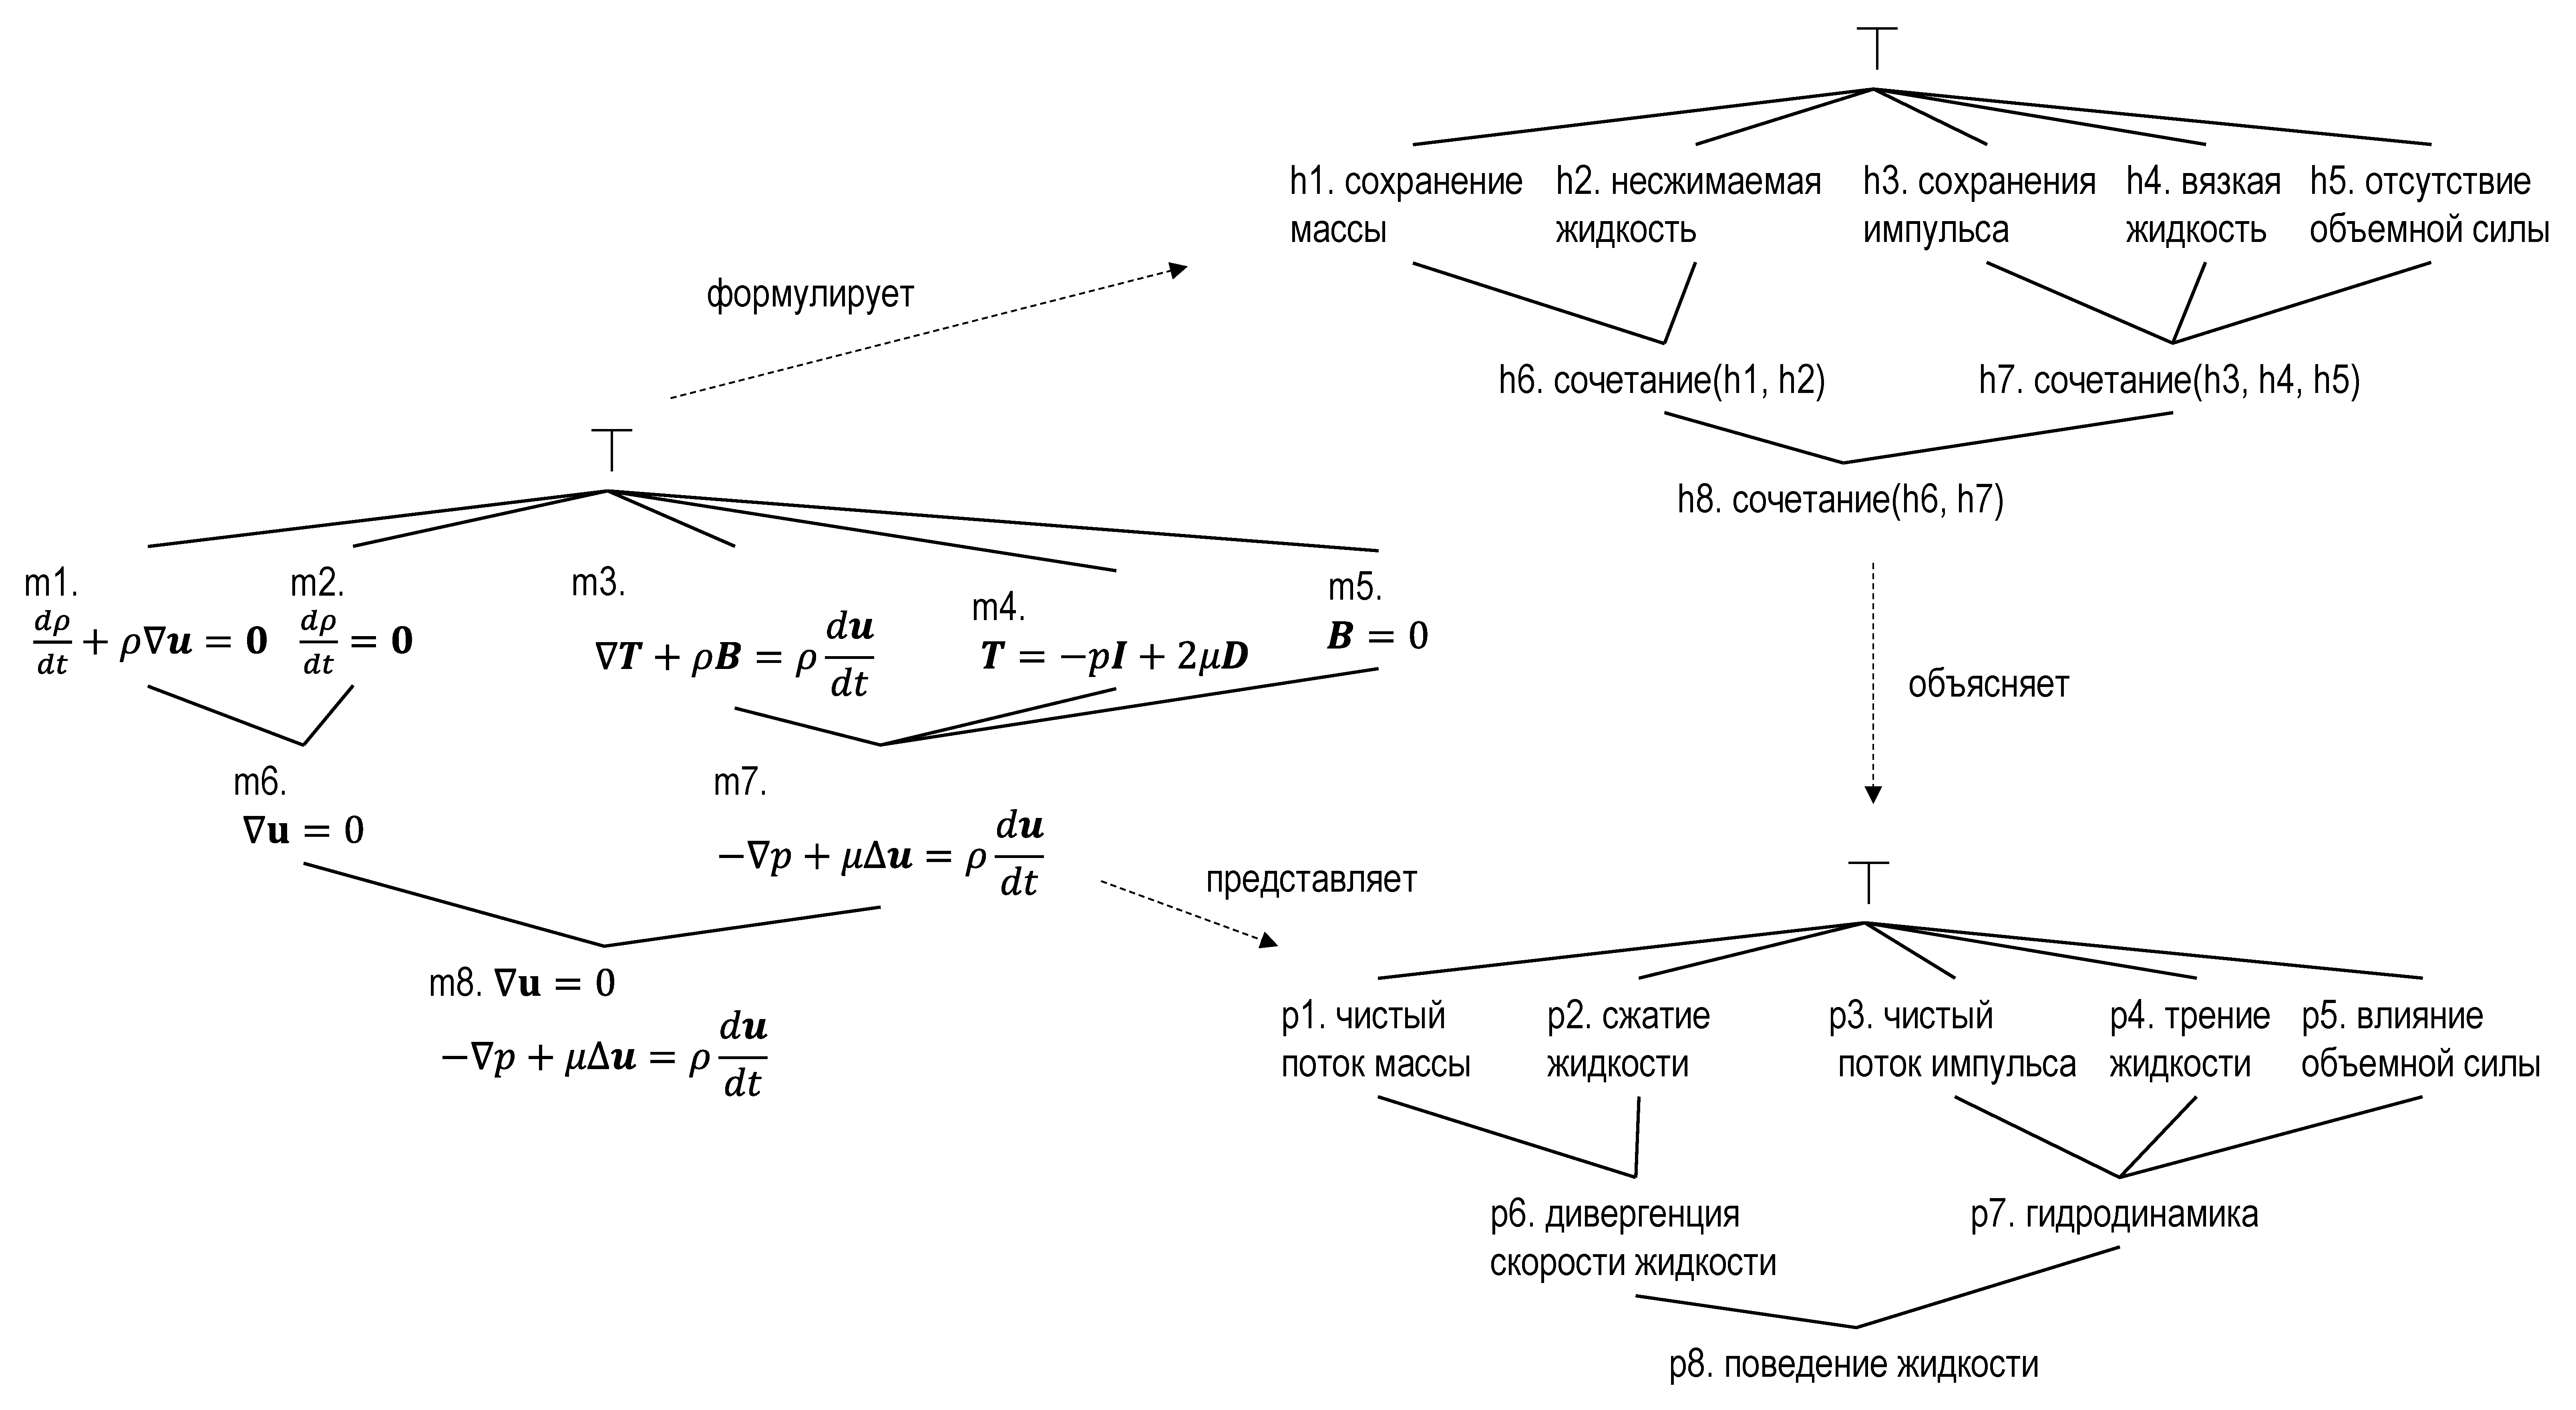
\includegraphics[width=1.0\linewidth]{images/lattice_fluid.pdf}
    \caption{Решетка гипотез, развернутая в модель, и изоморфная решётка явлений.}\label{fig:lattice_fluid}
\end{figure}

\textit{Модели} являются одним из основных инструментов современной науки. Модели могут выполнять две принципиально 
различные функции представления: модель может быть представлением выделенной части мира, или же модель может 
представлять определенную теорию в том смысле, как она (модель) интерпретирует законы и гипотезы данной теории.

Один из наиболее трудных вопросов в связи с моделями "--- это как они соотносятся с теориями. В этом плане модели 
могут рассматриваться как дополнения к теориям, как предварительные теории; они могут быть использованы в качестве 
замены теории, если теория слишком сложна для работы. Изучение модели ведется посредством прямых экспериментов, 
мысленных экспериментов и симуляции. Если задан набор параметров, модель может генерировать предполагаемые результаты 
относительно того, как система будет вести себя в конкретной ситуации. Модель и гипотезы, на которых она основана, 
укрепляются, если модель генерирует результаты, которые соответствуют поведению своего прототипа в реальном мире. 

\subsection{Проверка гипотез}\label{sect1_2_2}
Если научная гипотеза может быть проверена и опровергнута, она становится хорошей основой для дальнейшего 
моделирования. Для этого есть несколько способов, включая использование статистики, байесовского и логического вывода.
\subsubsection{Статистическая проверка гипотез}\label{sect1_2_2_1}
Для проверки и отбора гипотез применим как классический (частотный), так и байесовский статистический подход. 
Краткое изложение основных различий между этими подходами приведено ниже \cite{ivezic2019statistics}.

Классическая (частотная) статистика основана на следующих представлениях:
\begin{itemize}
    \item Вероятности "--- это относительные частоты событий. Они являются объективными свойствами объективного мира.
    \item Параметры гипотез (модели) являются фиксированными неизвестными константами. Поскольку они неизменны, 
            вероятностные утверждения относительно параметров не имеют смысла.
    \item Методы статистики должны иметь точно определенные долгосрочные частотные свойства.
\end{itemize}

После того как сформулированы нулевая и альтернативная гипотезы, необходимо принять некоторые статистические допущения 
относительно выборок данных, например, допущения о статистической независимости или распределения наблюдений. Если 
корректные допущения не приняты, это приводит к неверным результатам проверки.

Общая задача классической статистики "--- это задаться вопросом, согласуется ли данная выборка с гипотезой. Например, 
нас может интересовать, является ли результат измерения $x_i$ или даже целое множество $\{x_i\}$ согласуется с тем, 
что было выбрано из гауссова распределения $\mathcal{N}(\mu,\,\sigma^{2})$. Это \textit{нулевая гипотеза}.

Всегда принимается, что нам известно, как вычислить вероятность данного исхода на основе нулевой гипотезы: например, 
дана кумулятивная функция распределения, $0 \leq H_0(x) \leq 1$, тогда вероятность, что получается значение, 
по крайней мере, такое, как $x_i$, будет $p(x > x_i) = 1 $ "--- $H_0(x_i)$, и оно называется 
\textit{достигаемым уровнем значимости} $p$. Обычно принимается некоторый порог значения $p$, 
называемый \textit{уровнем значимости} $\alpha$, и нулевая гипотеза отвергается, если $p \leq \alpha $ 
(например, если $\alpha = 0.05$ и $p < 0.05$, нулевая гипотеза отвергается при уровне значимости $0.05$). 
Если гипотеза не отвергается, это не означает, что её корректность доказана, поскольку может оказаться, что объем 
выборки просто недостаточно велик для получения результата.

При выполнении такого рода проверок можно столкнуться с ошибками двух типов; статистики называют их 
\textit{ошибки I и II рода}. Ошибки I рода "--- это случаи, когда нулевая гипотеза верна, но несправедливо 
отвергнута. Применительно к поиску источников источники таких ошибок ложные, или, в более общем плане, такие 
результаты являются ложноположительными (в отношении альтернативной гипотезы). Вероятность ложноположительного 
результата при проверке единственного значения ограничивается принятым уровнем значимости $\alpha$. Случаи, когда 
нулевая гипотеза несправедлива, но не отвергается, называются ошибками II рода (недостаточные источники, или 
ложноотрицательные результаты (опять же в отношении альтернативной гипотезы)). Вероятность ложноотрицательного 
результата при проверке единственного значения обычно обозначается как $\beta$, и она связана с 
\textit{мощностью критерия} как $(1-\beta)$. Проверка гипотез тесно связана со сравнением распределений.

Если понизить уровень значимости $\alpha$ (критерий отбрасывания нулевой гипотезы становится более консервативным), 
количество ложноположительных результатов уменьшится, а количество ложноотрицательных увеличится. Таким образом, 
необходим компромисс, чтобы найти оптимальное значение $\alpha$, которое зависит от относительной важности 
ложноотрицательных и ложноположительных результатов для конкретной задачи. И одобрение ложных гипотез, и отбрасывание 
справедливых гипотез являются ошибками, которые исследователи должны стараться избегать. Существует дискуссия о том, 
какой случай \textit{менее} желателен; многие полагают, что всегда хуже, чем непринятие справедливой, и что наука 
должна в первую очередь стремиться избегать принятия ложных гипотез.

Если выполняется много случаев проверки гипотезы (такой процесс называется \textit{множественной проверкой гипотез}), 
доля ложноположительных результатов может существенно превысить значение $\alpha$. Доля ложноположительных результатов 
зависит не только от $\alpha$ и количества значений, но также и от количества справедливо положительных результатов 
(последнее пропорционально количеству случаев, когда альтернативная гипотеза справедлива). 

В зависимости от вида данных (дискретные или непрерывные случайные переменные), от того, что можно допустить (или нет) 
относительно лежащих в основе распределений, а также от конкретно поставленного вопроса, можно воспользоваться 
различными статистическими проверками. Исходная идея статистических тестов заключается в использовании данных для 
расчета надлежащей статистики и последующего сравнения полученного на основе данных значения с его ожидаемым 
распределением. Ожидаемое распределение оценивается \textit{в предположении, что нулевая гипотеза справедлива}. 
Если такое ожидаемое распределение подразумевает маловероятность того, что полученное на основе данных значение 
возникло случайно (т.е., соответствующее значение $p$ мало), то нулевая гипотеза отвергается с учетом пороговой 
вероятности $\alpha$, обычно 0.05 или 0.01 $(p < \alpha)$. Заметим еще раз, что $(p \geq \alpha)$ не означает 
\textit{доказанности} гипотезы.

Количество различных статистических тестов в литературе очень велико, и часто бывает трудно оценить их применимость 
(см. \cite{field2013discovering, wagner2019using}) в отношении разнообразия статистических методов в пакете 
статистических методов для социальных наук (Statistical Package for the Social Sciences "--- SPSS). Если распределения 
неизвестны, такие тесты называются непараметрическими. Наиболее популярным является тест Колмогорова-Смирнова, где 
проводится сравнение кумулятивного распределения функции $F(x)$ для двух выборок $\{x_{1i}\}, i = 1, \ldots, N_1$ и 
$\{x_{2j}\}, j = 1, \ldots, N_2$. Тест Колмогорова-Смирнова не является единственным вариантом для непараметрического 
сравнения распределений. Критерий Крамера–фон Мизеса, тест Ватсона и тест Андерсона-Дарлинга сходны с тестом 
Колмогорова-Смирнова, хотя и рассматривают несколько иную статистику. Тест Манна–Уитни–Вилкоксона (или критерий 
суммы рангов Вилкоксона) "--- непараметрический критерий для проверки того, получены ли два множества данных из 
распределений с разными параметрами положения (если известно, что эти распределения гауссовы, стандартный классический 
тест называется t-тестом). Можно воспользоваться несколькими стандартными классическими тестами, если известно или 
можно допустить, что $h(x)$ и $f(x)$ – гауссовы распределения (например, тест Андерсона–Дарлинга, тест Шапиро–Уилка). 
Дальнейшую информацию по статистическим тестам можно найти в \cite{ivezic2019statistics, field2013discovering, 
wagner2019using}.

\subsubsection{Выбор гипотезы (модели) и проверка в байесовском стиле}\label{sect1_2_2_2}

В отличие от частотного, байесовский подход принимает следующие допущения:
\begin{itemize}
    \item Вероятность указывает на степень субъективного убеждения, не ограниченного частотностью. Вероятностные 
        утверждения могут относиться не только к данным, но и к другим вещам, включая сами гипотезы (модели), а также к 
        их параметрам.
    \item Выводы относительно параметра делаются на основе его распределения вероятностей "--- такое распределение 
        дает количественную оценку неопределенности нашего знания относительно данного параметра. Различные точечные 
        оценки, как, например, математическое ожидание, могут быть затем легко получены из этого распределения.
\end{itemize}

Байесовская интерпретация вероятностей может рассматриваться как расширение логики высказываний (пропозиционной 
логики), которая позволяет рассуждения посредством гипотез, т.е. высказываний, чья справедливость или несправедливость 
не определены.

Байесовская вероятность относится к категории доказательственных вероятностей; чтобы оценить вероятность гипотезы, 
приверженец байесовской вероятности указывает некоторую априорную вероятность, которая впоследствии обновляется в 
свете новых релевантных данных (фактов) \cite{sivia2006data}. Байесовская интерпретация предоставляет стандартный 
набор методов и формул для выполнения таких расчетов.

Байесовский подход может рассматриваться как формализация процесса постоянного уточнения нашего знания об окружающем 
мире, начиная с отсутствия данных (состояние \textit{a priori}), и последующего совершенствования знания, умножая 
его вероятность по мере наблюдения данных в целях получения знания \textit{a posteriori}. Если рассматривается еще 
больший объем данных, то полученные из опыта апостериорные данные, основанные на первичном множестве данных, могут 
быть использованы в качестве априорных для вторичного анализа. Конечно, множества данных могут быть различными.

Нередко возникает вопрос: какую <<наилучшую>> модель (гипотезу) использовать? \textit{<<Выбор модели>>} "--- это 
методика, которой можно воспользоваться с целью провести грань между конкурирующими моделями (гипотезами) и выделить 
наилучшую модель (гипотезу) из некоторого множества ${M_1,\ldots, M_n}$, если есть определенные данные.

Необходимо напомнить базовую систему обозначений. Теорема Байеса может быть использована для расчета апостериорной 
вероятности $p(M_j|d)$ для каждой модели (или гипотезы) $M_j$, представляющей состояние нашего знания относительно 
справедливости модели (гипотезы) в свете данных $d$:

\begin{equation}
p(M_j|d) = \frac{p(d|M_j)p(M_j)}{p(d)} 
\end{equation}
где $p(M_j)$ "--- априорное понимание модели (гипотезы), которая представляет состояние нашего знания (или незнания) 
о справедливости модели (гипотезы) до начала анализа текущих данных, $p(d|Mj)$ "--- \textit{правдоподобность} модели 
(гипотезы), представляющая вероятность, что некоторые данные будут получены при допущении данной модели, 
и $p(d)$ "--- константа нормализации:

\begin{equation}
p(d) = \sum_{i} p\left( d|M_i\right) p(M_i)  
\end{equation}

Относительная <<приемлемость>> моделей получается сравнением апостериорных вероятностей; поэтому для сравнения двух 
моделей $M_a$ и $M_b$ рассматриваются отношение между апостериорными вероятностями моделей:

\begin{equation}
\frac{p(M_a|d)}{p(M_b|d)} = \frac{p(d|M_a)p(M_a)}{p(d|M_b)p(M_b)} 
\end{equation}

Коэффициент Байеса $B_{ab}$ может быть рассчитан как отношение правдоподобностей моделей:

\begin{equation}
B_{ab} = \frac{p(d|M_a)}{p(d|M_b)}
\end{equation}

Эмпирическая шкала на основе коэффициента Байеса $B_{ij}$ для оценки силы доказательств по двум моделям показана 
в \cref{tbl:bayescoef} \cite{march2011should}.

\begin{table} [ht]%
	\caption{Сила доказательств по двум моделям на основе коэффициента Байеса $B_{ij}$}%
	\label{tbl:bayescoef}% label всегда желательно идти после caption
    \setlength\extrarowheight{0pt} %вот этим управляем расстоянием между рядами, \arraystretch даёт неудачный результат
    \setlength{\tymin}{2.3cm}% минимальная ширина столбца
    \begin{center}

	\begin{tabulary}{\textwidth}{@{}>{\zz}C >{\zz}C >{\zz}L@{}}% Вертикальные полосы не используются принципиально, 
        % как и лишние горизонтальные (допускается по ГОСТ 2.105 пункт 4.4.5) % @{} позволяет прижиматься к краям
        \toprule     %%% верхняя линейка
    	$ |\ln B_{ij}| $ &
    	Соотношение ($\nu$) &
    	Мощность доказательства	\\
        \midrule %%% тонкий разделитель. Отделяет названия столбцов. Обязателен по ГОСТ 2.105 пункт 4.4.5 
        $<1.0$ &
        $<3:1$  &
        Недостаточное доказательство 
        \\
        \midrule
        $ 1.0 $ &
        $ ~3:1 $  &
        Слабое  доказательство 
        \\
        \midrule
        $2.5$ &
        $~12:1$  &
        Доказательство средней силы 
        \\
        \midrule
        $5.0$ &
        $~150:1$  &
        Сильное доказательство 
        \\
        \bottomrule %%% нижняя линейка
	\end{tabulary}%
 \end{center}
\end{table}

Коэффициент Байеса предлагает меру <<приемлемости>> модели независимо от более раннего представления о модели; 
чем больше коэффициент Байеса, тем лучше модель. Во многих случаях предварительное представление о каждой модели 
множества предлагаемых моделей будет одинаковым, тогда коэффициент Байеса будет эквивалентен соотношению апостериорных 
вероятностей моделей. <<Наилучшая>> модель в байесовском смысле "--- это та модель, которая наилучшим образом 
согласуется с данными в наименьшем параметрическом пространстве.

Особым случаем выбора модели (гипотезы) является \textit{байесовская проверка гипотезы} 
\cite{ivezic2019statistics, rouder2009bayesian}. Приняв $M_1$ как <<нулевую>> гипотезу, можно поставить вопрос: 
поддерживают ли данные альтернативную гипотезу $M_2$, т.е., можно ли отвергнуть нулевую гипотезу. Принимая априорные 
вероятности $p(M_1) = p(M_2)$ равными, получим отношение вероятностей

\begin{equation}
B_{21} = \frac{p(d|M_1)}{p(d|M_2)}  
\end{equation}

Невозможность отвергнуть $M_1$ в отсутствие альтернативной гипотезы весьма отлично от ситуации в процедуре проверки 
гипотезы в классической статистике. Последняя процедура отвергает нулевую гипотезу, если она не дает правильного 
описания данных, т.е. если очень маловероятно, что имеющиеся данные могут быть сгенерированы так, как предписывает 
нулевая гипотеза. Напротив, байесовский подход основан не на апостериорной вероятности данных, а на их апостериорной 
правдоподобности (вероятности), и не может отвергнуть гипотезу, если нет альтернативных объяснений наблюдаемых данных.

Сравнивая классический и байесовский подходы \cite{ivezic2019statistics}, трудно ожидать, что критически важный анализ 
будет выполнен в <<абсолютно байесовском>> стиле, т.е. без использования на разных стадиях частотных инструментов на 
разных стадиях процесса. Оставляя в стороне философию и красоту, можно сказать, что надежность вероятность и 
эффективность соответствующих вычислений при реализации байесовского подхода являются главными практическими вопросами. 
Центральным техническим вопросом, занимающим здесь основное место, является то, что значительно легче выполнить 
оптимизацию (надежно и эффективно) в больших размерностях, чем выполнить интегрирование. Так, используемые методы 
машинного обучения, хотя и прилагаются усилия адаптировать их к байесовской концепции, почти все основаны на 
частотных методах. 

Большинство из тех, кто применяет методы байесовской оценки, склонны на практике комплексно использовать байесовский 
и частотный инструментарий. Обратное также справедливо – частотные аналитики данных, хотя и остаются формально в 
рамках частотной концепции, нередко находятся под влиянием <<байесовского мышления>> относительно априорного и 
апостериорного. По-видимому, наилучшей рекомендацией может быть хорошее знание обеих парадигм, если требуется 
выносить информированные суждения о том, какие инструменты необходимо применять в той или иной ситуации. Дальнейшие 
сведения относительно байесовского подхода к проверке гипотез можно найти в \cite{ivezic2019statistics, sivia2006data, 
rouder2009bayesian}.

\subsubsection{Проверка гипотез c использованием логики}\label{sect1_2_2_3}
В соответствии с гипотетико-дедуктивным подходом гипотезы подвергаются проверке путем дедуктивного вывода прогнозов или 
иных эмпирических следствий из общих теорий. Если такие прогнозы проверяемы экспериментами, это поддерживает гипотезу. 
Необходимо отметить, что не все, из чего логически следует гипотеза, может быть подтверждено надлежащей проверкой. 
Соотношение между гипотезой и фактом часто не логическое, а эмпирическое. Чистая дедукция эмпирических следствий из 
гипотез, как это иногда бывает в физике, практически неприменима в биологии. Так, логическое следование фактов из 
проверяемых гипотез не является ни достаточным, ни необходимым для эффективной проверки. Вывод из наилучшего объяснения 
обычно интерпретируется как вид индуктивного вывода (см. рассмотрение абдукции в \ref{sect1_2_5_2}), когда 
объяснительные доказательства гипотезы принимаются в качестве показателя её справедливости \cite{weber2014}. 

Индуктивная логика есть система доказательной поддержки, которая расширяет дедуктивную логику до менее чем точных 
выводов. При правильной дедуктивной аргументации предпосылки логически влекут за собой заключение, где логическое 
следование означает, что справедливость предпосылок обеспечивают некоторую гарантию справедливости заключения. Точно 
так же при правильной индуктивной аргументации предпосылки должны обеспечивать некоторую степень поддержки заключения, 
причем такая поддержка означает, что справедливость предпосылок указывает на некоторую силу справедливости заключения. 
Если логика хорошей индуктивной аргументации предполагает реальную ценность, то мера поддержки, которую она выражает, 
должна удовлетворять <<критерию адекватности>> (CA): по мере накопления доказательств достигаемая степень, в которой 
набор справедливых доказательных утверждений поддерживает гипотезу, как показывают измерения в этой логике, должна 
стремиться показать, что гипотеза может быть, вероятно, несправедливой или, вероятно, справедливой. В работе 
\cite{hawthorne2021} подробно рассматривается степень, в которой такого рода логика, основанная на теореме Байеса, 
может давать оценку тому, насколько импликации гипотез относительно доказывающих фактов влияют на степень поддержки 
гипотез. В частности, показано, как такая логика может быть приложима к удовлетворению критерия CA: по мере 
накопления доказательств, несправедливые гипотезы будут, весьма вероятно, приобретать некоторые значения доказательной 
поддержки (измеряемые с помощью апостериорных вероятностей), приближающиеся к $0$; а когда это будет происходить, 
справедливая гипотеза будет, весьма вероятно, приобретать значения доказательной поддержки (измеряемые с помощью 
апостериорных вероятностей), приближающиеся к $1$.

\nomenclature{CO}{Criteria of Adequacy, критерий адекватности}

\subsection{Сравнение гипотез/моделей между собой} \label{sect1_2_3}

\subsubsection{Метрические подходы}\label{sect1_2_3_1}
Существует множество подходов к сравнению различных вычислительных моделей \cite{tirikov2021methods}. Одним из самых 
простых подходов \cite{pham2019new, pham2007system} является упорядочивание моделей по выбранной метрике на тестовых 
данных, например, среднеквадратичной ошибки или коэффициенту детерминации $R^2$. Преимуществом данного подхода 
является его простота, интерпретируемость и возможность сравнения моделей различных типов. К недостаткам данного
 подхода можно отнести невозможность определения лучшей модели из нескольких при несовпадении порядка метрик моделей 
 на разных наборах данных, а также невозможность оценки общности модели и ее устойчивости при добавлении новых данных 
 или изменении существующих. Этот подход в основном применяется для отсечения моделей с целью уменьшения в дальнейшем 
 числа попарных сравнений, а также для ранжирования моделей по выбранной метрике.

Вторым подходом к сравнению различных вычислительных моделей является использование статистической проверки гипотез. 
Для данного подхода формулируются нулевая и альтернативная гипотезы, экспертом выбирается уровень значимости, задается 
статистика с известным распределением при верности нулевой гипотезы. В зависимости от проверяемой гипотезы экспертом 
выбирается статистический тест и вычисляется достигаемый уровень значимости. По результатам сравнения достигаемого 
уровня значимости с изначально выбранным значением отвергается или не отвергается нулевая гипотеза. Данный способ 
сравнения наиболее распространён для моделей, зависящих линейно от своих параметров \cite{pham2007system}. Например, 
если одна из моделей является вложенной в другую модель, то проверяется гипотеза о равенстве параметров двух 
рассматриваемых моделей. Более общим является сравнение разности между предсказаниями двух моделей для поиска 
статистически значимого различия \cite{rencher2008linear}. В работе \cite{mahmoudi2018testing} для сравнения моделей 
на схожесть используется статистический тест, который проверяет гипотезу о равенстве нулю медианы разности предсказаний 
двух рассматриваемых моделей. В качестве статистического теста использованы критерий Уилкоксона и критерий знаков. 
В работе \cite{tirikov2021methods} критерий знаков используется для попарного сравнения двух множеств нелинейных моделей. 
Обычно этот подход применяется для попарного сравнения моделей на схожесть их предсказаний.

Третьим подходом к сравнению различных вычислительных моделей является использование методов, разработанных в рамках 
теории информации. Преимуществом такого подхода является возможность оценить не только качество предсказания модели, 
но также и степень её переобучения. Одним из самых распространённых является информационный критерий Акаике 
\cite{akaike1974new}. Критерий подходит для сравнения моделей, построенных не только из данных, но и теоретических 
моделей. Например, в статье \cite{liddle2007information} использован критерий Акаике для сравнения астрономических 
моделей. Критерий Акаике вычисляется по следующей формуле:

\nomenclature{AIC}{Akaike information criterion, Критерий Акаике}
\nomenclature{BIC}{Bayesian information criterion, Байесовский информационный критерий}


\begin{equation}
AIC=2k-2\ln L
\end{equation}

где $k$ "--- это число настраиваемых параметров модели, а $L$ "--- это функция максимального правдоподобия вычислительной 
модели. Лучшей из нескольких моделей считается та, которая имеет наименьшее значение \textit{AIC}. Недостатком данного 
метода является его плохая применимость на выборках малого размера. 

Преодолеть данный недостаток позволяет использование модифицированного информационного критерия Акаике:  
\begin{equation}
AICc = AIC + \frac{2k^2+2k}{n-k-1}
\end{equation}
где $n$ "--- это размер выборки. Модифицированный критерий является менее общим и применим при условии, что модель 
линейно зависима от своих параметров. Второе слагаемое накладывает штраф за большое количество настраиваемых параметров 
при малом объеме выборки. 

Другим информационным критерием является использование информационного критерия Байеса: 
\begin{equation}
BIC_I= 2k \ln n - 2\ln L
\end{equation}

где $k$ "--- это число настраиваемых параметров модели, $L$ "--- это функция максимального правдоподобия вычислительной 
модели, а $n$ "--- это количество значений в выборке. Основное отличие от критерия Акаике состоит в том, что 
накладывается более строгое ограничение на число настраиваемых параметров. Информационный критерий является 
применимым, если $n \gg k$ \cite{tarasov2017estimation}. Подход с использованием информационных критериев применяется 
для сравнения моделей различной природы, а также для отсечения моделей большого размера.

Для некоторых моделей, например, построенных генетическим программированием, рекомендуется использовать 
модифицированный критерий Акаике и Байеса, учитывающий особенности применяемого алгоритма 
\cite{giraud2021introduction}.  Информационный критерий Акаике и Байеса для моделей генетического программирования 
вычисляются следующим образом:

\begin{equation}
  \begin{array}{l}
AIC=\epsilon_n (m) + \frac{2h}{n} \sigma^2  \\
BIC=\epsilon_n (m) + \frac{h}{n} \sigma^2 \ln n  
  \end{array}
\end{equation}

где $h$ обозначает сложность модели, $n$ "--- количество значений в выборке, $\epsilon_n (m)$ "--- эмпирическая ошибка, 
$\sigma^2$"--- дисперсия ошибки.

Четвертым подходом к сравнению вычислительных моделей является использование байесовского подхода 
(см. \cref{sect1_2_2_2}). Идея данного подхода заключается в переходе от априорных знаний к апостериорным с учетом 
наблюдаемых данных. Вначале вычисляется разность предсказаний двух моделей. Затем проверяется гипотеза о том, что 
среднее вычисленной разности равно нулю. Байесовский критерий в данном случае будет выглядеть следующим образом:

\begin{equation}
\Lambda(X) = \frac{\prod_{i=1}^n \frac{2}{\sigma\sqrt{2\pi}} * \exp{\left(-\frac{\left(x_i - \mu\right)^2 }
    {2\sigma^2}\right)}}{\prod_{i=1}^n \frac{2}{\sigma\sqrt{2\pi}} * \exp{\left(-\frac{\left(x_i \right)^2 }
    {2\sigma^2}\right)}} < \eta
\end{equation}
где $\mu$ аппроксимируется из данных. Если неравенство  выполняется, то нулевая гипотеза не отвергается. Преимуществом 
байесовского подхода является возможность определения степени уверенности по $ \eta $ в проверке гипотезы по 
\cref{tbl:bayescoef}. Применение информационных критериев используется для ранжирования моделей по качеству их 
предсказания и сложности, позволяет сравнивать модели различной природы.

Пятым подходом к сравнению вычислительных моделей является поиск схожести графового представления моделей 
\cite{wang2018direct}. Данный метод сравнивает похожесть двух ориентированных ацикличных графов, строя разностный 
ориентированный ацикличный граф. При этом делается предположение, что графы задаются линейной моделью структурных 
уравнений. Данный метод отличается от других тем, что с его помощью можно сравнивать две различные системы в 
совокупности. Преимуществом данного подхода является возможность аппроксимации разностного графа без явного построения 
изначальных графов.  Недостатком данного подхода является экспоненциальная вычислительная сложность построения 
разностного графа и невозможность учесть скрытые переменные. Подход применяется, если модель представима в виде графа 
и служит дополнительной проверкой при оценке схожести моделей.

\subsubsection{Байесовская мотивация открытия}\label{sect1_2_3_2}
Один из способов выбора между конкурирующими моделями явления "--- использовать байесовской подход к селекции модели 
(\cref{sect1_2_2_2}), где байесовские доказательства справедливости каждой из предложенных моделей (гипотез) могут быть 
рассчитаны, а модели могут быть ранжированы по степени их байесовской доказанности. Это хороший метод для выявления 
наилучшей модели данного множества моделей, однако он не дает никакого указания на абсолютную пригодность 
(доказанность) модели. Байесовская селекция моделей ничего не говорит об общем качестве множества моделей (гипотез) 
в целом "--- наилучшая модель множества может просто оказаться наилучшей в множестве плохих моделей. Знание того, что 
наилучшая модель в данном множестве моделей не является особенно хорошей моделью всегда дает мотивацию к поиску лучшей 
модели и, следовательно, может привести к открытию модели.

Один из способов установить некоторую меру абсолютной пригодности модели – использовать понятие байесовского сомнения, 
впервые введенного в работе \cite{starkman2008introducing}. Байесовское сомнение оперирует сравнением всех известных 
моделей в пределах множества с идеальной моделью, которая принимается как эталонная.

Применение метода байесовского сомнения для построения космологической модели представлено в работе 
\cite{march2011should, march2013advanced}. Один из самых важных вопросов космологии "--- определение фундаментальной 
модели, подкрепляющей огромное количество доступных на сегодняшний день наблюдений. Так называемая <<согласованная 
космологическая модель>> основана на космологическом принципе (т.е. на том, что Вселенная изотропна и однородна, 
как минимум, в достаточно большом масштабе) и сценарии горячего Большого взрыва, за которым последовала эпоха инфляции. 
Эту в достаточной степени простую модель можно объяснить с помощью всего лишь нескольких 
свободно-параметрических наблюдений, 
охватывающих гигантский масштаб времени и пространства. Поскольку необходимо, чтобы и холодная темная материя (CDM), 
и космологическая константа ($\Lambda$) удовлетворяли имеющимся данным, согласованную модель часто 
называют <<моделью $\Lambda$CDM>>. 

\nomenclature{CMD}{Cold dark matter, холодная темная материя}

Несколько различного типа объяснений возможны для наблюдаемого более позднего ускорения [расширения] Вселенной, включая 
различные классы моделей темной энергии, напр., $\Lambda$CDM, $\omega$CDM, теории изменяющейся гравитации, модели 
вакуума или обратной реакции \cite{march2011should}. Методология байесовского сомнения, которая дает абсолютную 
степень совершенства модели, применялась к вопросу о том, следует ли сомневаться в модели $\Lambda$CDM.

Методология байесовского сомнения требует введения неизвестной идеализированной модели $M$, с которой можно было бы 
сравнивать все другие модели. Как следует из работы \cite{starkman2008introducing}, <<сомнение>> может быть определено 
как апостериорная вероятность неизвестной модели:

\begin{equation}
 D \equiv p(M|d) = \frac{p(d|M)p(M)}{p(d)}
\end{equation}

Здесь $p(M)$ – априорное сомнение, т.е. априорная вероятность неизвестной модели, которая представляет собой степень 
уверенности в том, множество известных моделей не содержит достоверной модели. Сумма априорных вероятностей всех 
моделей должны быть равна единице. Методология байесовского сомнения требует наличия базисной модели (наилучшей модели 
в множестве известных моделей), в качестве которой в данном случае была выбрана модель $\Lambda$CDM. Усредненный 
коэффициент Байеса по модели $\Lambda$CDM и каждой из известных моделей может быть представлен как:

\begin{equation}
<B_{i\Lambda}> \equiv \frac{\sum_{i=1}^N B_{i\Lambda}}{N}
\end{equation}

Отношение $R$  между апостериорным и априорным сомнением, которое называется относительным изменением сомнения, 
выражается как:

\begin{equation}
R \equiv \frac{D}{p(M)}
\end{equation}

Чтобы сомнение выросло, т.е. чтобы апостериорное сомнение было больше априорного ($R \ll 1$), коэффициент Байеса 
с учетом неизвестной модели X и базисной модели должен быть много больше, чем усредненный коэффициент Байеса:

\begin{equation}
\frac{<B_{i\Lambda}>}{B_{M\Lambda}} \ll 1
\end{equation}

Чтобы серьезно усомниться в базисной модели $\Lambda$CDM, недостаточно, что $R > 1$; вместе с этим вероятность 
$\Lambda$CDM также должна снизиться, чтобы её апостериорная вероятность была больше её априорной вероятности, т.е. 
$p(\Lambda|d) < p(\Lambda)$. Определим

\begin{equation}
R_\Lambda \equiv \frac{p(\Lambda|d)}{p(\Lambda)}
\end{equation}

Чтобы поставить $\Lambda$CDM под сомнение, необходимо выполнить следующие два условия:
\begin{equation}
R > 1, R_\Lambda < 1
\end{equation}

Если они выполняются, это предполагает, что множество известных моделей не является полным, и создает мотивацию к 
поиску лучшей модели, пока еще не включенной во множество, что может привести к открытию. В работе 
\cite{starkman2008introducing} предложен способ расчета абсолютной верхней оценки для $p(d|M)$, которая может быть 
достигнута в классе известных моделей. В довершение к этому было обнаружено, что космический микроволновой фон (CMB), 
энергетический спектр материи (matter power spectrum "--- MPS) и наблюдения сверхновых типа Ia (SNIa) не требуют 
введения альтернативной модели в базисную модель $\Lambda$CDM. Верхняя оценка байесовского доказательства пока 
неизвестной модели темной энергии в противовес $\Lambda$CDM дает лишь слабое свидетельство в пользу неизвестной модели. 
Поскольку речь идет об абсолютной верхней оценке, был сделан вывод о том, что $\Lambda$CDM остается достаточным 
феноменологическим описанием имеющихся наблюдений.

\nomenclature{CMB}{Cosmic microwave background, космический микроволновой фон}
\nomenclature{MPS}{matter power spectrum, энергетический спектр материи}
\nomenclature{SNIa}{Type Ia Supernova, Cверхновая типа Ia}


\subsection{Оценка параметров гипотез/моделей} \label{sect1_2_4}
Модели (гипотезы) обычно описываются параметрами $\boldsymbol{\theta}$, значения которых оцениваются на основе данных. 
Здесь этот процесс описывается в соответствии с \cite{ivezic2019statistics}. Для конкретной модели $M$ и априорной 
информации $I$ получаем:

\begin{equation}
    p(M, \boldsymbol{\theta}|d, I) = \frac{p(d|M, \boldsymbol{\theta}, I) p(M, \boldsymbol{\theta} |I)}{p(d|I)}
\end{equation}

Результат $p(M, \boldsymbol{\theta}|d, I)$ называется функцией \textit{апостериорной} плотности вероятности (pdf) 
для модели $M$ и параметров $\boldsymbol{\theta}$ для известных данных $d$ и другой априорной информации $I$. 
Это "--- $(k + 1)$-размерная pdf в пространстве, охватываемом $k$ параметрами модели и моделью $M$. Член 
$p(d|M, \boldsymbol{\theta}, I)$ "--- \textit{правдоподобность} (вероятность) данных для \textit{известной} 
модели $M$ и фиксированных значений описывающих её параметров $\boldsymbol{\theta}$, а также всей другой 
априорной информации $I$. Член $p(M, \boldsymbol{\theta}|I)$ "--- априорное совместное распределение вероятностей 
для модели $M$ и её параметров $\boldsymbol{\theta}$ в отсутствие каких-либо данных, используемых для расчета 
правдоподобности (вероятности), и априорным распределением (prior).

В байесовской формуле $p(M, \boldsymbol{\theta}|d, I)$ соответствует состояние нашего \textit{знания} (т.е., 
представления) о модели и её параметрах при известных данных $d$. Для простоты обозначение $M(\boldsymbol{\theta})$ 
будет заменяться на $M$ всегда, когда отсутствие явной зависимости от $\boldsymbol{\theta}$ не будет приводить к 
недоразумениям. Байесовский анализ данных проходит следующие концептуальные этапы:

\begin{enumerate}
    \item Формулировка вероятности данных $p(d|M, I)$.
    \item Выбор априорного распределения вероятностей $p(\boldsymbol{\theta}|M,I)$, которое включает в себя все 
            другие знания, которые могут существовать, но \textit{не} используется при расчете вероятностей (например, 
            априорные измерения одного и того же типа, различные измерения или просто неинформативное априорное 
            распределение). Было предложено несколько методов построения <<объективных>> априорных распределений. Один из 
            них "--- \textit{принцип максимальной энтропии} для сопоставления неинформативных априорных распределений 
            путем максимизации энтропии по подходящему множеству pdf, нахождение распределения, которое наименее 
            информативно (при условии заданных ограничений). Максимизация энтропии в отсутствие проверяемой информации 
            производится с одним ограничением: сумма вероятностей должна быть равна $1$. При этом ограничивающем 
            условии максимальная энтропия для дискретного распределения вероятностей задается однородным распределением.
    \item Определение апостериорного распределения $p(M|d, I)$ с использованием теоремы Байеса. На практике для сложных 
            многомерных задач этот этап может оказаться вычислительно-ёмким.
    \item Поиск параметров наилучшей модели $M$, которые максимизируют $p(M|d, I)$ и дают \textit{максимальную 
            апостериорную} (MAP) оценку. Такая \textit{точечная оценка} является естественным аналогом максимальной 
            оценки вероятности (MLE) в классической статистике.
    \item Квантификация неопределенности оценок параметров посредством использования \textit{доверительных интервалов}. 
            Как и оценка MLE, такая оценка может быть получена аналитически путем математических расчетов, специфичных 
            для выбранной модели. Так же, как и для MLE, для симулирования выборок из апостериорного распределения 
            можно выбирать различные цифровые методы. Это можно рассматривать как аналог частотного подхода, где можно 
            симулировать выборки из лежащих в основе достоверных распределений данных. В обоих случаях по таким 
            выборкам могут быть произведены различные расчеты описательной статистики для рассмотрения 
            неопределенностей, охватывающих данные, а также оценки параметров модели, основанных на этих данных.
    \item \textit{Проверка гипотезы}, необходимая для получения других выводов относительно 
            модели (гипотезы) или оценок параметров.
\end{enumerate}


\subsection{Порождение гипотез в научных экспериментах}\label{sect1_2_5}
\subsubsection{Формульное и алгоритмическое моделирование}\label{sect1_2_5_1}
Существуют две культуры анализа данных (формульное моделирование  и алгоритмическое моделирование в соответствии с 
работой \cite{breiman2001statistical}), которые могут быть применимы для порождения гипотез, основанных на данных. 
Формульное моделирование "--- это процесс оценки соотношений между переменными. Он включает в себя многочисленные методы 
моделирования и анализа нескольких переменных, сосредоточенных на формулах $y = f\left(\Vec{x}\right)$, которые и дают 
отношение, определяющий вектор зависимых переменных $y$ в соответствии с вектором независимых переменных $x$. 
В экспериментальной статистике (основанной на различных методах регрессии) зависимая переменная определяет изучаемое 
событие и ожидается, что она будет изменяться всегда, когда меняется независимая переменная (прогнозные переменные, 
сторонние переменные). Такие методы, как линейная регрессия, логистическая регрессия, множественная регрессия являются 
хорошо известными примерами, представляющими соответствующий подход к моделированию.

В культуре алгоритмического моделирования соответствующий подход заключается в поиске алгоритма, который оперирует 
на $x$ для прогнозирования реакций $y$. Наблюдается множество значений $x$ на входе и результирующее множество 
значений $y$ на выходе. Точность прогноза и свойства алгоритмов (такие, напр., как их сходимость, если они итеративны) 
являются вопросами, которые необходимо исследовать. Алгоритмы машинного обучения сосредотачиваются на предсказании, 
основанном на известных свойствах, полученных из данных. Такие алгоритмы, как деревья принятия решений, ассоциативное 
правило, нейронные сети, метод опорных векторов, как и другие методы обучения в байесовских и вероятностных моделях 
\cite{barber2012bayesian, hastie2009elements} представляют собой примеры, связанные со второй культурой. 

Модели, которые наилучшим образом эмулируют природу в отношении точности прогнозирования, являются также и наиболее 
сложными и малопонятными. Природа продуцирует выходные значения y из входных значений x при посредстве черного ящика 
со сложной и неизвестной внутренней частью. Существующие в настоящее время точные методы прогнозирования также 
являются сложными черными ящиками (напр., нейронные сети, множества деревьев (графов), опорные векторы). Таким образом, 
мы сталкиваемся с двумя черными ящиками, где наш ящик представляется всего лишь немного более проницаемым, чем черный 
ящик природы \cite{breiman2001statistical}. Выбирая между точностью и интерпретируемостью, человек на практике 
предпочитает интерпретируемость. 

Целью модели, однако, является не интерпретируемость (как способ получения информации), а получение полезной и точной 
информации о соотношении между реакцией и прогностическими переменными. В работе \cite{breiman2001statistical} 
показано, что алгоритмические модели могут обеспечивать более высокую точность предсказания, чем формульные модели, 
предоставляя также дополнительную информацию относительно лежащего в основе механизма. Реально это именно то, что 
является целью статистического анализа. Исследователям необходимо сосредоточится на решении задач вместо того, чтобы 
задаваться вопросом, какую регрессионную модель они могут создать. 

Возражением против этого тезиса (предложенного Коксом) является то, что прогнозирование без некоторого понимания 
лежащего в основе процесса и связывания его с другими источниками информации становится все более и более 
неопределенным. Поэтому предлагается строить модели стохастических расчетов, которые дают обобщённое понимание 
изучаемого явления. Одной из целей такого подхода может быть некоторое понимание и проверка гипотез о лежащем в основе 
процессе. Если будет дан относительно небольшой объем выборки, такое направление могло бы быть продуктивным. 
Однако характеристики данных быстро меняются. Во многих наиболее интересных современных задачах, предложение начинать 
с формальной модели неубедительно. Методы, используемые в статистике, неприменимы для выборок небольшого объема и 
небольшого количества переменных. Средства анализа данных должны быть более прагматичными. Если поставлена 
статистическая задача, необходимо найти хорошее решение, будь то формульная модель, алгоритмическая модель, 
байесовская модель или совершенно иной подход. В контексте анализа, движимого гипотезами, необходимо обратить внимание 
на вопрос о том, насколько далеко можно зайти в применении алгоритмического моделирования в генерации и проверке 
гипотез. В машинном обучении используются различные подходы относительно формирования и выбора гипотез; их можно найти 
в \cite{barber2012bayesian, breiman2001statistical, ivezic2019statistics}.

Кроме машинного обучения, интересный пример алгоритмической генерации гипотез можно найти в проекте <<IBM Ватсон>> 
\cite{ferrucci2010building}, где симбиоз технологий (1) универсальной обработки естественного языка (NLP) многократного 
пользования и (2) представления знаний и логических суждений (KRR) под названием DeepQA используется для ответа на 
произвольные вопросы по существующим документам на естественном языке, а также по структурированным информационным 
ресурсам. Процесс генерации гипотез использует результаты анализа вопроса и выдает потенциальные ответы путем поиска 
доступных источников данных и извлечения подходящих ответов как фрагментов результата поиска. Каждый потенциальный 
ответ, сопоставленный с вопросом, рассматривается в качестве гипотезы, которую система должна доказать с некоторой 
степенью достоверности. После сопоставления гипотез система должна их ранжировать и оценить их достоверность по общей 
шкале. Подход, принятый в машинном обучении, основан на прогоне системы через набор тренировочных вопросов с известными 
ответами и обучения модели с учетом оценок по той же шкале. При работе с программами, дающими оценки по шкале NLP, 
существенно то, что возможности, которые они предоставляют, могут быть довольно скудными, и поэтому точная оценка 
достоверности требует применения взвешенной по достоверности техники обучения \cite{ferrucci2010building} – нового 
класса онлайновых методов обучения, которые поддерживают вероятностную меру достоверности каждого параметра. Важно 
отметить, что вместо проверки гипотез на основе статистики для шкальной оценки различных вопросов (гипотез) и 
интерпретаций контента применяется контекстная оценка большого ряда свободно связанной вероятностной аналитики контента 
на базе вопросов и семантики. Обучение разных моделей на разных объемах данных одновременно, а также объединение 
полученных машиной классификаторов в единый классификатор позволяет выработать процесс, применимый к большим базам 
данных. Дальнейшие подробности можно найти в работах \cite{ferrucci2010building, dredze2008confidence}, а также в 
других публикациях, связанных с проектом <<IBM Ватсон>>. 

\subsubsection{Генерация гипотез при помощи логического вывода}\label{sect1_2_5_2}
Ученые, которые поддерживают рациональность научных открытий, представили несколько методов генерации гипотез, включая 
открытие как абдукцию, индукцию, обнаружение аномалий, эвристическое программирование и использование 
аналогий \cite{Woodward2011}.

\textit{Открытие как абдукция} характеризует процессы умозаключений, которые происходят до момента, когда 
подтверждается новая гипотеза. Абдуктивная модель рассуждений, которая приводит к формулированию правдоподобных гипотез, 
концептуализируется как вывод, начинающийся с данных. В соответствии с работой \cite{nickles1980scientific} абдукция 
происходит следующим образом:

\begin{enumerate}
    \item есть некоторые явления $p_1, p_2, p_3, \ldots $, которым объяснения нет или оно недостаточно;
    \item однако явления  $p_1, p_2, p_3, \ldots $ наблюдаются, и будет неудивительно, если появится гипотеза $H$. 
            Явления, конечно, будут следовать чему-то подобному гипотезе $H$ и будут объясняться ею; 
    \item Таким образом, есть все основания разрабатывать гипотезу $H$ "--- чтобы предложить ее в качестве возможной 
            гипотезы, допускающей $p_1, p_2, p_3, \ldots $. Абдуктивная модель рассуждений, в основном, является 
            процессом объяснения аномалий или необычных явлений \cite{Schickore2014}. Рассуждения ученого абдуктивно 
            переходят от аномалии к объяснительной гипотезе, в свете которой данные явления уже не будут необычными. 
            Может существовать несколько различных гипотез, которые объясняют явления, в результате чего возникает 
            необходимость в дополнительных критериях для выбора между различными гипотезами.
\end{enumerate}

Одним из способов внедрения абдуктивной модели рассуждения является абдуктивное логическое программирование 
\cite{Kakas1992}. Генерация гипотез в рамках абдуктивной логики организована следующим образом. Например, в процессе 
эксперимента наблюдаются некоторые новые наблюдения. Пусть $B$ представляет собой фоновые знания; $O$ "--- множество 
фактов, представляющих наблюдения. Как $B$, так и $O$ – логические программы (набор правил на некотором языке правил). 
Кроме того, $\Gamma$ обозначает множество литералов, представляющих собой множество абдуктивностей (abducibles) "--- 
потенциальных допущений для добавления к $B$ с целью объяснения $O$. Если имеются $B, O$ и $\Gamma$, то задача 
генерации гипотез заключается в нахождении такого множества литералов $H$ (называемого гипотезой), что: 

\begin{enumerate}
    \item $B$ и $H$ определяют $O$;
    \item $B$ и $H$ совместимы;
    \item $H$ является подмножеством $\Gamma$.
\end{enumerate}


Если все условия удовлетворяются, то H является объяснением O (по отношению к $B$ и $\Gamma$).  Примеры систем 
абдуктивного логического программирования включают в себя <<ACLP>> \cite{Kakas2000}, <<A-system>> \cite{Nuffelen2001}, 
<<ABDUAL>> \cite{Alferes2004} и <<ProLogICA>> \cite{Ray2006}. Абдуктивное логическое программирование может быть также 
выполнено с помощью систем программирования, основанных на программировании 
наборов ответов ASP (Answer Set Programming), например, с помощью систем <<DLV>> \cite{Leone2006}. 

\nomenclature{ASP}{Answer Set Programming, программирование наборов ответов}

Пример абдуктивной логической программы в <<ProLogICA>> описывает простую модель метаболизма лактозы у бактерии 
\textit{E. coli} \cite{Ray2006}. Фоновые знания B показывают, что \textit{E. coli} может питаться лактозой (молочным 
сахаром), если бактерия производит два фермента, пермеазу и галактозидазу. Как и все ферменты (\textit{E}), эти 
ферменты выделяются, если они кодируются экспрессированным геномом (\textit{G}). Эти ферменты кодируются двумя генами 
(\textit{lac(y)} и \textit{lac(z)}) в генном кластере (\textit{lac(X)}), называемым опероном, который экспрессирован, 
когда уровень (\textit{amt}) глюкозы низок, а уровень глюкозы высок, или же когда оба уровня средние. Абдуктивности 
\textit{Г}, показывают, что все основные случаи предикатов \textit{amount} допустимы. Этим выражается тот факт, что 
в модели уровни различных веществ в каждый момент неизвестны. Это "--- неполная информация, которую требуется  
уточнить в каждой рассматриваемой нами задаче. Ограничения целостности требуют, чтобы уровень вещества (\textit{S}) 
может иметь только одно значение.

\begin{ListingEnv}[!h]% настройки floating аналогичны окружению figure
    \captiondelim{ } % разделитель идентификатора с номером от наименования
    \caption{Порождение новых гипотез с использованием логики предикатов}\label{list:generation}
    % окружение учитывает пробелы и табуляции и применяет их в сответсвии с настройками
    \begin{lstlisting}[language={Prolog}]
    %  Фоновые знания (B) 
    feed(lactose) :- make(permease), make(galactosidase).
    make(Enzyme) :- code(Gene,Enzyme), express(Gene).
    express(lac(X)) :- amount(glucose, low), 
                        amount(lactose, hi).
    express(lac(X)) :- amount(glucose, medium),
                        amount(lactose, medium).
    code(lac(y), permease).
    code(lac(z), galactosidase).
    temperature(low) :- amount(glucose, low).
    false :- amount(S, V1), amount(S, V2), V1 != V2.
    
    %  Абдуктивности (Г)
    abducible_predicate(amount).
    
    % Наблюдение (O)
    feed(lactose).

    % Порождаются две гипотезы:
    {amount(lactose, hi), amount(glucose, low)}
    {amount(lactose, medium), amount(glucose, medium)}
    \end{lstlisting}
\end{ListingEnv}%

Еще пара других примеров реальных основанных на правилах систем, где используется абдуктивное логическое 
программирование. Робот-ученый (см. \cref{sect1_3_2}) абдуктивно создает гипотезу новых фактов относительно 
функциональной биологии дрожжей, делая вывод о том, чего не хватает в модели \cite{King2011}. В работе 
\cite{TamaddoniNezhad2006} абдукция и индукция используются для формулирования гипотез относительно угнетения 
метаболических путей. С помощью абдукции осуществляется прибавление фоновых знаний, после чего для изучения общих 
правил используется индукция. В работе \cite{Inoue2009} авторы применяют систему умозаключений <<SOLAR>> для 
абдуктивной генерации гипотез относительно подавляющего влияния токсинов на метаболизм крыс.

Процесс открытия имеет также глубокую связь с поиском аномалий. Есть много методов и алгоритмов для выявления аномалий. 
Обнаружение аномалий является важной исследовательской задачей анализа данных, нацеленного на поиск объектов, которые 
существенно различны, исключительны и противоречат большей части информации во входной базе данных \cite{Bartha2013}.

% \textit{Аналогии} играют в науке несколько ролей. Они не только вносят свой вклад в открытия, но также и играют свою 
% роль в развитии и оценке научных теорий (новых гипотез) путем рассуждений по аналогии.

\subsubsection{Генерация гипотез из публикаций в биоинформатике}\label{sect1_2_5_3}
Имея целью быстрый анализ и проверку гипотез, исследователи и ученые ведущих академических, фармацевтических и 
других исследовательских центров начали использовать <<Куратор открытий Ватсона (Watson Discovery Advisor)>> от <<IBM>>, 
используя данные миллионов научных работ в общедоступных базах данных. 

Опираясь на способности <<Ватсона>> разбираться в нюансах натурального языка, <<Куратор открытий Ватсона>> способен 
понимать язык науки, напр., как взаимодействуют химические соединения, что превращает его в уникально мощный инструмент 
исследователей в медико-биологические науках и других областях исследования и промышленности. В области 
медико-биологических наук <<Куратор открытий Ватсона>> располагает объёмом специальных знаний и понимает 
узкоспециализированный лексикон в таких областях, как данные клинического исследования, геномика, лекарственные 
препараты и анатомия человека.

Ученые из Бэйлорского медицинского колледжа и <<IBM>>, используя основанный на технологии <<Ватсона>> <<Бэйлорский 
инструментарий интеграции знаний (Baylor Knowledge Integration Toolkit KnIT)>>, нашли новые ферменты 
(называемые киназами), которые могли бы модифицировать особый белок \textit{p53}, имеющий отношение ко многим видам 
рака \cite{spangler2014automated}. Имеется свыше 240\,000 публикаций в соответствующих аннотациях медицинской базы 
данных <<Медлайн>>, где упоминаются одна или более из 500+ известных киназ человека. <<Ватсон>> выполнил анализ 70\,000 
научных статей по \textit{p53}, чтобы дать предварительную оценку белков, которые включают или выключают работу 
\textit{p53}. Такой автоматизированный анализ привел к тому, что онкологи из Бэйлора выделили шесть потенциальных 
киназ \textit{p53} для нового исследования. Эти результаты примечательны, поскольку за последние 30 лет ученым 
удавалось сделать открытие в среднем только одной киназы \textit{p53} в год. Знание того, какие именно белки 
модифицируются каждой киназой, и, таким образом, на какие киназы будут хорошо действовать препараты, является трудной и 
пока не решенной проблемой. Есть свыше 500 известных киназ человека и десятки тысяч возможных белков, на которые 
можно <<нацелиться>>. 

<<KnIT>> подбирает аннотации для извлечения информации путем запросов данных. В этом процессе используются название 
определенной киназы и её синонимов. Разрешение запроса по существу ведется следующим образом. Слова и фразы, включенные 
в признаковое пространство документов, определяются подсчетом количества документов, в которых появляется каждое слово 
и выявлением слов, получивших максимальный счет. Последовательность двух слов рассматривается как фраза. Отбирается 
только $N$ наиболее частых слов и фраз. Это становится признаковым пространством. Когда признаковое пространство 
сформировано, создается представление каждой киназы усреднением признаковых векторов всех документов, содержащих 
данную киназу. Это центроид каждой киназы. Далее рассчитывается матрица расстояний, куда помещаются измерения 
расстояний между каждой киназой каждой другой киназой в признаковом пространстве.

Наконец, получена наполненная смыслом картина отношений между киназами. Теперь есть возможность найти набор киназ, 
которые могут модифицировать \textit{p53}. С тем чтобы приоритизировать киназы для дальнейших экспериментов, 
необходимо, однако, иметь некоторую принципиальную схему ранжирования. Для получения такой схемы был применен метод 
диффузии графов \cite{zhou2003learning}. Диффузия графов является подходом к обучению для классификации, основанной 
на размеченных и неразмеченных данных. Необходима известная информация (начальные метки), которая затем ограничивает 
новые метки, чтобы обеспечить их гладкость в отношении определенной структуры (напр., сети). В нашем случае нам 
известно, какие киназы могут модифицировать \textit{p53} (начальные метки); нам желательно знать, какие другие белки 
могут модифицировать \textit{p53} (конечные метки). Матрица расстояний, основанная на опубликованных данных, дает нам 
структуру сети киназ. Начальные метки извлекаются из текущей информации, находящейся в обзорных статьях.

Для проверки данного алгоритма он был вначале применен в ретроспективном анализе, чтобы выяснить, могут ли недавние 
аннотации по новым киназам \textit{p53}, появившиеся после определенного срока, могли бы быть предсказаны на основе 
модели, которая принимала во внимание только работы, написанные до этого времени, когда упомянутые открытия киназ 
\textit{p53} были еще неизвестны. Затем был поставлен вопрос, могут ли некоторые вариации алгоритма улучшить 
прогнозирование киназ \textit{p53}, для чего его эффективность сравнивалась с общим подходом, обычно принятом в 
биологии для идентификации функционально подобных белков. И наконец, анализ был расширен для охвата большего набора 
белков, чтобы проверить его масштабируемость.

Это исследование является первым этапом совместной работы <<IBM>> "--- <<Бэйлор>> и в таком качестве подтверждает 
установку, что извлечение информации из опубликованных ранее материалов является жизнеспособной стратегией 
прогнозирования ранее неизвестных биологических фактов. Было показано, что киназы \textit{p53}, предсказанные методами 
извлечения информации из текстов, поддерживаются лабораторными результатами. В будущем станет возможно делать и многие 
другие виды предсказаний в значительно большем масштабе, поскольку инфраструктура и возможности расширятся. Планируется 
в будущем сосредоточиться на более обширной области белков и функций, наращивая всеобъемлющие сети взаимодействий и 
предсказывая, где должны существовать новые связи, на основе всего остального, что известно. Можно ожидать, что этот 
процесс в конце концов ускорит скорость появления открытий в онкологии на целый порядок и позволит ученым прийти к 
значительно более полному пониманию механизмов такого рода заболеваний. Применении <<KnIT>> в других областях биологии 
или естественных наук не является простым и ясным. Например, обобщение, включающее в себя большее количество белков и 
генов, уже является серьезной задачей. В таких дисциплинах, как физика, результаты, как правило, представляются в форме 
уравнений и графов, а не текстов. Тем не менее, группы, занимающиеся извлечением информации, работают над получением 
информации также и из этих представлений.


\section{Средства поддержки экспериментов, движимых научными гипотезами}\label{sect1_3}

\subsection{Движимые гипотезами роботы. Робот-ученый Адам}\label{sect1_3_1}
<<Робот-ученый>> \cite{king2009automation, sparkes2010towards}, ориентированный на геномные приложения, 
является физически реализованная система, которая способна выполнять циклы научных экспериментов и делать 
открытия полностью автоматически: формирование гипотез, выбор экспериментов для проверки этих гипотез, выполнение 
экспериментов на базе робототехнической системы, анализ и интерпретация результатов, повторение цикла (система с 
обратной связью, в которой полученные результаты используются для научения и передачи полученного в результате знания 
снова в экспериментальные модели). Дедукция, индукция и абдукция "--- это виды логического рассуждения, используемого 
в научном открытии (см. \cref{sect1_2}). Полная автоматизация науки требует обучения в системе с обратной связью, где 
компьютер не только анализирует результаты, но и научается на них и отправляет полученные в результате знания назад, 
в следующий цикл процесса (\cref{fig:RobotScientistCycle}).

\begin{figure}[ht]
    \centering
    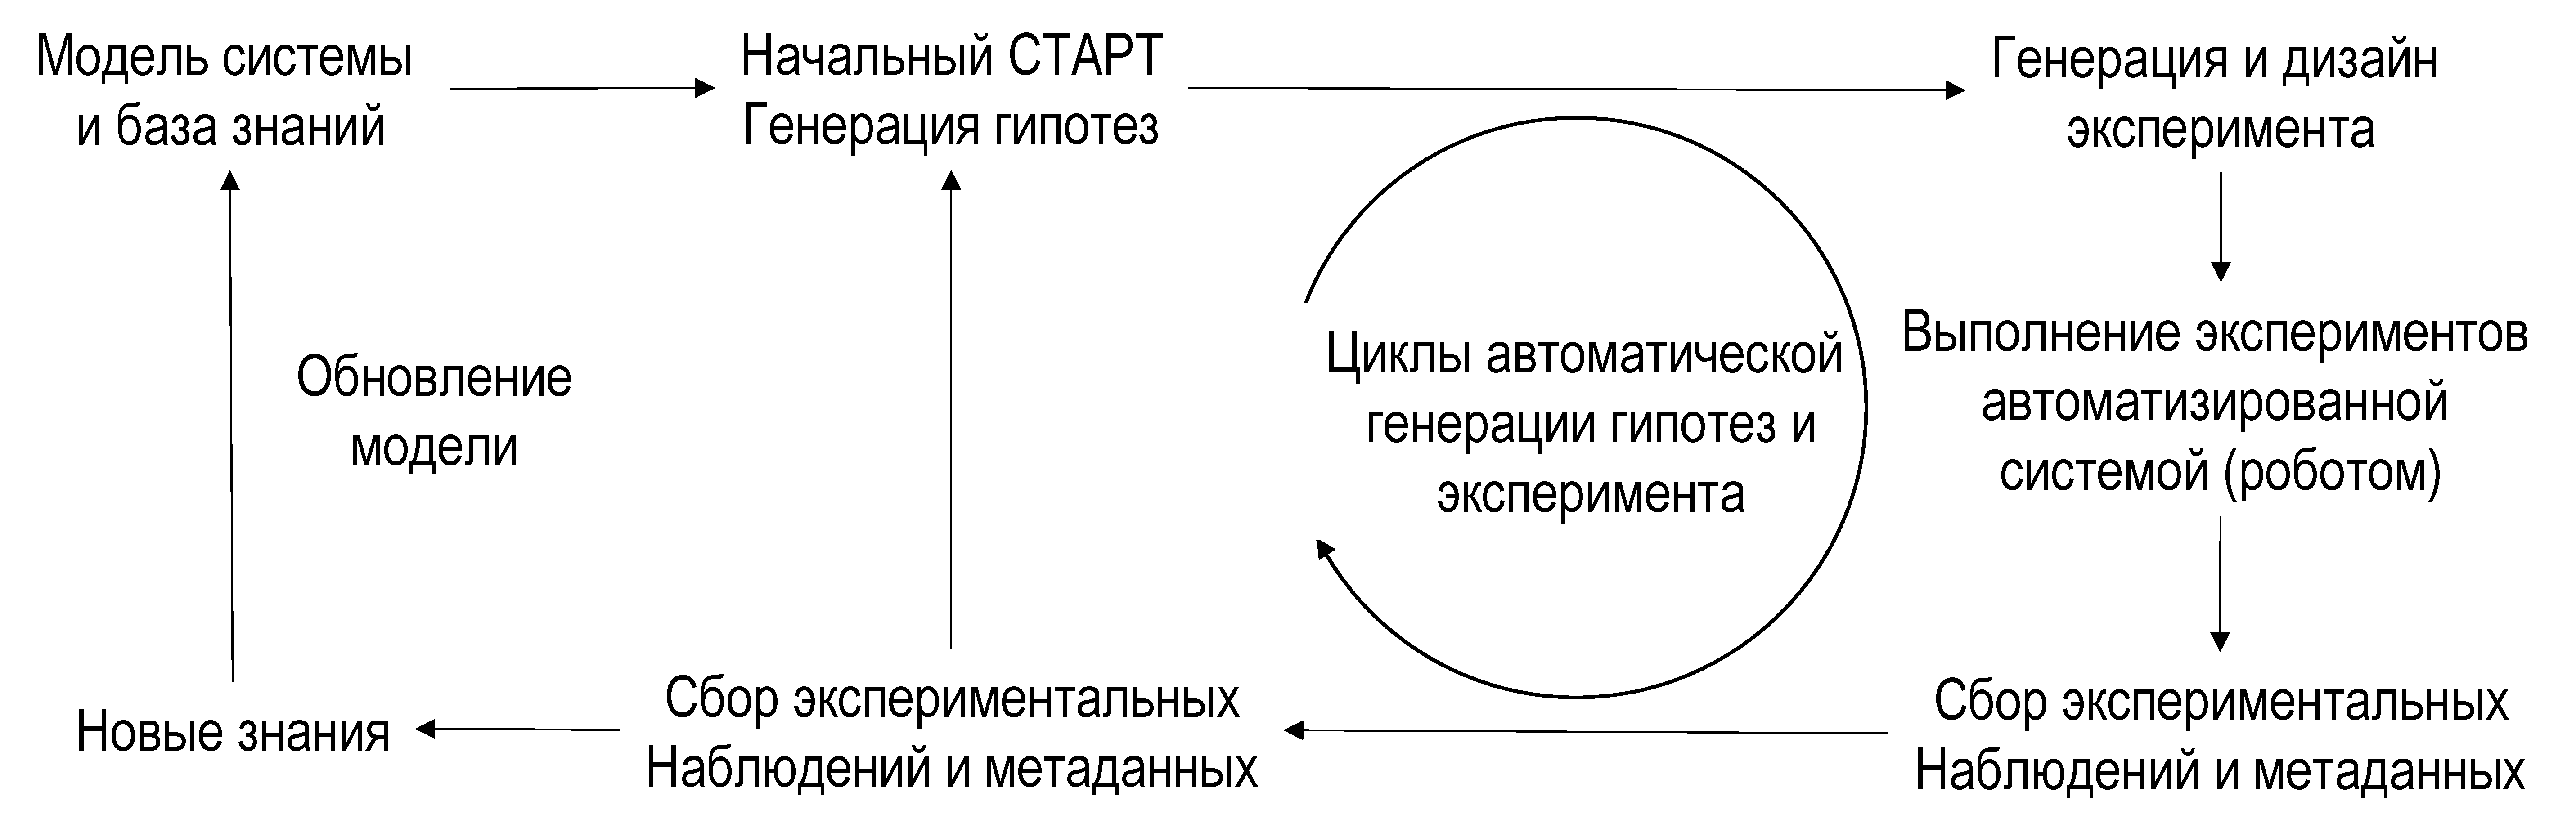
\includegraphics[width=1.0\linewidth]{images/RobotScientistCycle.pdf}
    \caption{Воплощение гипотезы.}\label{fig:RobotScientistCycle}
\end{figure}

У <<Робота-ученого>> автоматизированное формирование гипотез основывается на следующих ключевых компонентах:

\begin{enumerate}
    \item Рассчитываемое машиной представление знаний в данной области.
    \item Абдуктивный или индуктивный вывод новых гипотез.
    \item Алгоритм селекции гипотез.
    \item Дедукция экспериментальных следствий из гипотез.
\end{enumerate}	

<<Адам>>, первый прототип <<Робота-ученого>>, был разработан с целью выполнения экспериментов по выращиванию микробов 
и изучения функциональной геномики дрожжевых грибков \textit{Saccharomyces cerevisiae}, точнее говоря, для выявления 
генов, кодирующих <<местно орфанные ферменты>>. <<Адам>> использует всеобъемлющую логическую модель метаболизма дрожжей в 
сочетании с биоинформационной базой данных (<<Kyoto Encyclopaedia of Genes and Genomes (KEGG) – Киотская энциклопедия 
генов и геномов) и стандартной биоинформационной методикой поиска гомологий (<<PSI-BLAST>> и <<FASTA>>) для выдвижения 
гипотез о вероятно потенциальных генах, которые могут кодировать местно орфанные ферменты. Это абдуктивный процесс 
генерации гипотез.

С целью формализации экспериментов, проводимых <<Адамом>> в направлении функциональной геномики, была разработана 
онтология <<LABORS>> (<<Лабораторная онтология для <<Роботов-ученых>>). <<LABORS>> является версией онтологии <<EXPO>> (как 
верхний слой онтологии), приспособленной для представления биологических знаний <<Роботам-ученым>>. <<LABORS>> выражен 
на языке OWL DL. <<LABORS>> определяет различные структурные подразделения исследований, напр., испытание, собственно 
исследование, цикл исследований и воспроизведение, а также разработка стратегии, конфигурация пластины, реально 
ожидаемые результаты. Также определяются соответствующие понятия и отношения в данных функциональной геномики и 
метаданных. Как <<LABORS>>, так и соответствующие базы данных (используемые для хранения случаев в пределах классов) 
переводятся на язык Datalog для обеспечения возможности пользования механизмом рассуждения SWI-Prolog в необходимых 
приложениях \cite{king2004functional}
.
Генерировались два уровня (вида) гипотез. Первый уровень связывает орфанный фермент, представленный своим номером 
класса ферментов (\textit{E.C.}), с геном, который (\textit{ORF}), возможно, его кодирует. Это отношение выражается 
как двухместный предикат, где первый аргумент "--- \textit{ORF}, а второй "--- номер \textit{E.C.} Пример гипотезы 
на этом уровне: \textit{encodesORFtoEC('YBR166C', '1.1.1.25')}.

Второй уровень гипотез учитывает связь между конкретным штаммом, указываемым по имени отсутствующего в нем \textit{ORF}, 
и химическим соединением, которое должно влиять на рост штамма, если в его среду добавляется питательное вещество. На 
этот уровень гипотеза выходит из первого путем логического вывода с использованием специфической модели дрожжевого 
метаболизма. Пример такой гипотезы: (влияет на рост) \textit{affects\textunderscore growth('C00108', 'YBR166C')}, где 
первый аргумент "--- химическое вещество (названия соответствуют <<KEGG>>), а второй аргумент "--- рассматриваемый штамм. 
Затем <<Адам>> проектирует экспериментальные анализы, необходимые для проверки гипотез в роботизированной лабораторной 
системе. Эксперименты основаны на двухфакторном решении, в котором проводится сравнение множественных репликатов 
анализируемых штаммов (с метаболитами и без) и диких штаммов-контролей (с метаболитами и без).

<<Адам>> работает в рамках гипотетико-дедуктивного метода (\cref{sect1_2_5}). <<Адам>> абдуктивно предполагает новые факты 
относительно функциональной биологии дрожжей, затем дедуктивно выводит экспериментальные выводы из этих фактов, 
используя свою модель метаболизма, которые затем проверяет в экспериментах. С целью выбора экспериментов <<Адам>> 
принимает во внимание переменные затраты на эксперименты, а также различные вероятности гипотез. <<Адам>> выбирает 
свои эксперименты с учетом минимизации ожидаемых затрат на исключение всех гипотез, кроме одной. В целом, это 
\textit{NP}-полная задача, и <<Адам>> находит решение эвристически \cite{soldatova2011representation}.

По-видимому, в настоящее время большинство гипотез в биологии генерируется компьютерами. Компьютеры всё более 
автоматизируют процесс формирования гипотез; в химии, напр., программы машинного обучения (на основе индукции) 
используются для помощи в создании лекарственных препаратов, а в биологии аннотация геномов "--- это, в сущности, 
масштабный процесс (абдуктивного) формирования гипотез. Такие компьютерно-генерируемые гипотезы, конечно, выражены в 
доступной для вычислений форме, однако вносить их в общедоступную базу данных, предоставляя для других приложений, 
пока еще не стало общей практикой \cite{soldatova2011representation}.

Подробности разработки формализации, используемой <<Адамом>> в исследованиях функциональной геномики, можно найти в 
работах \cite{qi2010ontology,soldatova2011representation}. Основанная на онтологии формализация, базирующаяся на 
теории графов и логическом моделировании, дает возможность безошибочно отслеживать блоки результатов, используемые 
для разных целей, сохраняя семантику всех логических категорий экспериментов, вовлеченных в полный объем исследований. 
Показано, как используются эксперименты и машинное обучение для выработки дополнительного знания в целях 
усовершенствования модели метаболизма.

В системе используются: 

\begin{enumerate}
    \item метод логического вывода новых гипотез при проведении экспериментов на основе абдуктивного логического 
            программирования для генерации достоверных гипотез, объясняющих наблюдения;
    \item метод статической оценки корректности соответствия гипотез полученным данным.
\end{enumerate}

Пользователям разрешается использовать новые метаданные для эксперимента (например, свой дизайн эксперимента). 
С использованием этого дизайна система автоматически пытается с помощью логического вывода породить новые 
гипотезы и проверить их. Дополнительно система позволяет подобрать оптимальный набор входных параметров 
итеративно на небольшом количестве начальных экспериментов, которые проводятся с различным выбором 
экспериментальных параметров.

\subsection{Гипотезы как данные в вероятностных базах данных}\label{sect1_3_2}
Еще один взгляд на кодирование и обработку гипотез представлен в работе \cite{GoncalvesP14}. Авторы работы используют 
методы вероятностных баз данных для систематического построения и обработки гипотез. Вероятностная система обработки 
баз данных <<MayBMS>> \cite{huang2009maybms} является ядром обработки гипотез. Эта методика (называемая 
<<$\Upsilon$"---DB>>) дает возможность исследователям поддерживать несколько гипотез, объясняющих некоторые явления, 
и предоставляет основанный на байесовском подходе механизм оценки для ранжирования гипотез.

Построение базы данных <<$\Upsilon$"---DB>> включает в себя несколько этапов (см. \cref{fig:Upsilon_db_pipeline}). 
На первом этапе логические категории явлений и гипотез предлагаются как входные данные системы. Гипотеза является 
системой математических уравнений, выраженных в виде функций в формате W3C MathML; она ассоциируется с одним или не 
одним набором данных для испытания методом симулирования, где наборы данных состоят из последовательностей из $n$ 
кортежей с входными переменными уравнения и его соответствующего выхода в виде функционально зависимых \textit{FD} 
переменных (прогнозов, или предикторов). 

\begin{figure}[ht]
    \centering
    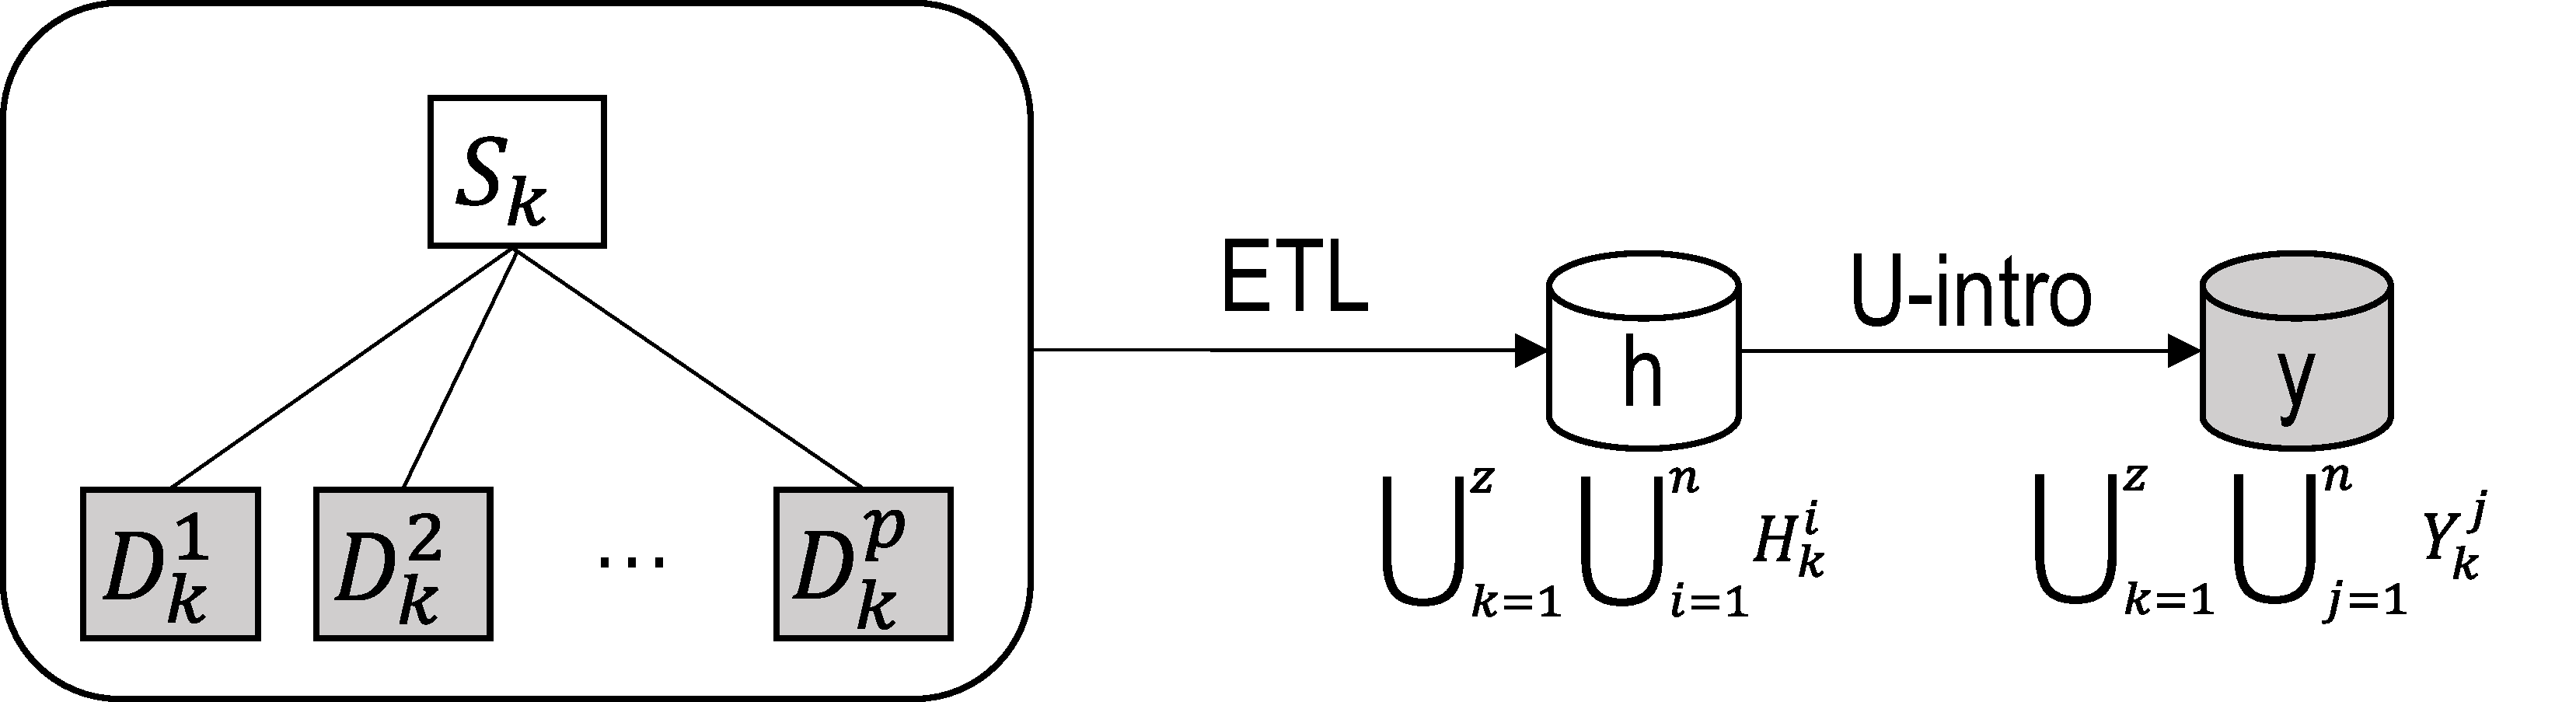
\includegraphics[width=0.7\linewidth]{images/Upsilon_db_pipeline.pdf}
    \caption{Этапы кодирования гипотез как данных в вероятностных базах данных.}\label{fig:Upsilon_db_pipeline}
\end{figure}

Явление представлено, по меньшей мере, одной эмпирической базой данных, подобной базам данных для испытания методом 
симулирования. На следующем этапе система работает с гипотезами и явлениями следующим образом: 
\begin{enumerate}
    \item исследователь должен предоставить некоторые метаданные относительно гипотез и явлений; напр., гипотезы должны 
            быть связаны с соответствующими явлениями и им должно быть приписано априорное распределение достоверности 
            (по умолчанию однородное в соответствии с принципом максимальной энтропии (\cref{sect1_2_5}));
    \item из уравнений извлекаются функциональные зависимости \textit{FD}, с тем чтобы получить схему базы данных для 
            хранения симуляций и экспериментальных данных; следует отметить, что для точного определения формулировок 
            гипотез в \textit{FD} вводятся особые атрибуты-ссылки на явления и гипотезы; 
    \item кортежи (последовательности из n членов) получаются из результатов симуляционных испытаний и наблюдательных 
            данных путем неопределенного псевдотранзитивного замыкания и логических рассуждений;
    \item наконец, формируется вероятностная база данных <<$\Upsilon$"---DB>>. Если явление и гипотеза 
            (с эмпирическими наборами данных и симуляционными испытаниями) представлены, становится возможным 
            манипулировать ими с помощью интструментов базы данных.
\end{enumerate}

В системе при добавлении нового набора данных для всех гипотез в системе, для которых этот набор данных является 
актуальным, пересчитывается байесовская вероятность. При этом ее предыдущее значение считается априорной вероятностью, 
а по новым данным вычисляется апостериорная вероятность. При добавлении новой гипотезы в систему в виде системы 
уравнений сначала система производит ее формальное кодирование гипотез в качестве кортежей базы данныъх, а затем 
вычисляется оценка соответствия гипотез наборам данных.

В системе в качестве основных методов можно выделить:
\begin{enumerate}
    \item формальное кодирование гипотез в качестве кортежей баз данных (представление гипотез в виде систем 
            уравнений над кортежами базы данных);
    \item оценка соответствия гипотез наборам данных;
    \item построение причинно-следственных зависимостей для параметров одной гипотезы.
\end{enumerate}

Система <<MayBMS>> обеспечивает инструменты для оценки конкурирующих гипотез, объясняющих явление. Когда имеются 
априорные вероятности, система дает возможность сделать еще один или не один (если появляются новые данные наблюдений) 
шаг для байесовского вывода. На каждом этапе априорная вероятность обновляется, становясь в соответствии с теоремой 
Байеса апостериорной. Как результат, гипотезы, лучше объясняющие данное явление, получают более высокие вероятности, 
дающие возможность исследователям делать более достоверные заключения (см. также \cref{sect1_2_4}). 
Подход <<$\Upsilon$"---DB>> обеспечивает перспективный путь анализа гипотез в области масштабных ИИИД, являясь 
непостоянной прогнозирующей (предикторной) базой данных, учитывающей эмпирические данные.


\subsection{Система поддержки научных исследований <<Гефест>>}\label{sect1_3_3}
В основе системы <<Гефест>> (Hephaestus) \cite{Duggan2015} лежит работа с виртуальными экспериментами над данными. 
Система помогает исследователю искать корреляционные зависимости между большим числом переменных, предоставляет 
возможность сформировать гипотезы по наиболее перспективным связям, а затем с помощью тщательного тестирования перейти 
к причинно-следственной зависимости. 

Система позволяет исполненять виртуальный эксперимент над существующими базами данных, которые могут выполнять 
некоторую аналитику локально. Она ориентирована на работу с очищенными и размеченными данными. Система состоит из 
следующих модулей:
\begin{itemize}
    \item Компонент для работы с наборами данных. Авторы стремятся создать некую поисковую систему, которая принимает 
            на вход строку, описывающую параметры гипотезы, возвращает ранжированный список потенциальных 
            причинно-следственных зависимостей.
    \item Компонент тестирования гипотез. Является основным компонентом системы. Движок составляет запрос для оценки 
            каждого возможного взаимодействия, разбивает образцы на контрольные блоки и высчитывает заданную метрику 
            точности для каждого из них. После расчета статистики для блока, движок объединяет результаты, получая 
            взвешенную оценку гипотезы.
    \item Компонент ранжирования результатов. Гипотезы объединяются и сортируются по некоторой вероятностной оценке.
\end{itemize}

Центральным блоком системы является SQL-подобный декларативный язык для описания виртуального эксперимента, 
с помощью которого возможно проектировать дизайн эксперимента, специфицировать основные гипотезы и их параметры, 
тестировать их, исполнять выбранные эксперименты и публиковать исследования. Так как применение только статистических 
методов и машинного обучения может приводить к ошибочным результатам в поиске причинно-следственных связей, то системы 
ориентирована на симбиоз между человеком и машиной. Используя корреляционные связи, которые были проверены экспертами 
в предметной области, <<Гефест>> собирает вероятностно причинные графы для спецификации семантики предметной области. 
Причинный граф поддерживает большое количество связей, обнаруженных в процессе выполнения виртуального эксперимента, 
а также позволяет исследовать последовательность выявления вероятностных причин и аномалий. Система позволяет отсекать 
некоторые неперспективные вычислительные маршруты c точки зрения конечных метрик, 
минимизируя общее количество вычислений.

Основными методами для манипулирования гипотезами и виртуальными экспериментами являются:
\begin{enumerate}
    \item метод автоматического порождения гипотез из данных "--- символьная регрессия при подборе аппроксимирующей 
            формулы для выбранного подмножества переменных на наборе данных;
    \item метод интервенций при исполнении виртуального эксперимента - установление существующих и возможной 
            генерации новых гипотез, которые значимо влияют на выбранную экспертом гипотезу;
    \item метод корректного разбиения данных наблюдений при проверке статистических гипотез для обеспечения 
            несмещенных оценок при дальнейшем тестировании гипотез;
    \item метод ранжирования нескольких конкурирующих гипотез, наиболее соответствующих наблюдениям, 
            по выбранной метрике (например, достигаемому уровню значимости) или нескольким метрикам;
    \item метод построения графа причинно-следственных и вероятностных зависимостей для оценки соответствия 
            полученных зависимостей общепринятым в области, а также для потенциального исследования значимых 
            корреляций и их последующего преобразования в причинно-следственные зависимости.
\end{enumerate}

При добавлении нового набора данных или объединении нескольких разрозненных наборов данных применяется следующая 
процедура. Система вычисляет выбранные метрики точности каждого набора данных независимо и вычисляет их взвешенную 
сумму для последующей оценки гипотезы. Разработчик эксперимента сам выбирает весовую функцию. При этом рекомендуется 
учитывать такие факторы, как размер или дисперсия выборки каждого набора данных. Система в автоматическом режиме не 
выполняет слияние всех наборов данных в один большой набор. Так как разные наборы данных могут содержать не все 
переменные, то система с использованием линейной регрессии может построить зависимость отсутствующих переменных по 
другим наборам данных и восстановить их при необходимости, если это требуется для корректной оценки гипотезы.

\subsection{Не гипотезо-ориентированные системы}\label{sect1_3_4}

Система FCCE \cite{schales2015fcce} предназначена для поиска корреляций в неоднородных наборах данных, охватывающих 
большие диапазоны времени. Ключевым компонентом модели данных является концепция функций. Функции определяют отношение 
между ключом и некоторым значением, каждый элемент которого может содержать несколько функций. FCCE представляет 
упрощенную модель реляционных данных для пользователя, где каждая таблица хранит один тип характеристики. Каждая 
строка идентифицируется по ключу и может содержать несколько функций. В системе FCCE ключевым методом является 
построение попарных корреляционных зависимостей для всех переменных множества разрозненных наборов данных. Для метода 
существует распределенная реализация, позволяющая искать значимые корреляции между разнообразным набором данных разных 
типов, при этом используются различные временные окна. Данная система рассматривалась на примере двух задач из области 
безопасности: обнаружения доменных имен потенциальных сетей зараженных рабочих станций и пост-инцидентное расследование 
проникновения. Для минимизации задержек обработки данных решено было отказаться от использования традиционных 
реляционных баз данных для хранения информации и перейти на NoSQL. Ключевым компонентом модели данных является 
концепция признаков. Признаки определяют связь между парой ключ-значение, каждый элемент из которых может содержать 
несколько атрибутов. FCCE представляет упрощенную реляционную модель данных для пользователя, где каждая таблица хранит 
один тип признаков. Каждая строка идентифицируема ключом и может содержать несколько атрибутов. FCCE обеспечивает 
API для хранения, получения и вычисления корреляции над признаками. Разработчики предлагают оригинальный подход 
интеграции модуля оценки критерия корреляции в движок исполнения запросов над хранилищем, позволяющий ускорить время 
ответа на запрос и снизить накладные расходы на вычисление и вводвывод. FCCE использует два отличительных механизма 
для поддержки эффективности операций нахождения корреляций между признаками: канал запросов и модификатор запросов. 
Канал "--- механизм, позволяющий передавать признаки, извлеченные из одного запроса в другой запрос в качестве входных 
данных, т.е. последовательно можно объединять несколько GET функций, тем самым создавай пересечения нескольких 
признаков. Модификатор – над GET запросом предполагает использование широкого набора опций для более тонкого контроля 
его поведения.

%TODO недостатки SDI
Платформа SDI \cite{demchenko2013addressing}  используется для поддержки научных экспериментов. Система может 
интегрировать открытые данные, повторно использовать данные наблюдений и данные моделирования при эволюции виртуальных 
экспериментов. SDI требует поддержки происхождения, классификации, индексации экспериментов и данных, полного цикла 
получения данных, их обработки и очистки, создания экспериментов для проверки гипотез над большими коллекциями данных, 
агрегирования результатов в течение продолжительных периодов времени. Платформа также позволяет интегрировать открытые 
данные, повторно использовать данные наблюдений и данные моделирования при эволюции виртуальных экспериментов. 
Вместе с тем, SDI не позволяет непосредственно работать с гипотезами, не устанавляваются зависимости между гипотезами 
в одном эксперименте.

MLCask \cite{Luo2021} "--- это git-подобная ветвящаяся система, предназначенная для обработки нелинейных моделей 
машинного обучения и конвейеров данных. Это позволяет совместно разрабатывать конвейер и повторно использовать 
промежуточные результаты вычислений для сокращения продолжительности операции слияния на основе выбранной метрики. 
Система не имеет прямого отношения к понятию гипотезы и каким-либо взаимозависимостям между ними. Кроме того, проверка 
гипотез не является частью системы.

MLflow \cite{Zaharia2018} и Dagster \cite{Dagster2022} "--- это программные пакеты, которые предоставляют API для 
выполнения конвейеров машинного обучения. Позволяет хранить кэшированные результаты выполнения функции. Эти системы 
позволяют отслеживать выполнение на предмет происхождения, повторного использования конфигурации, а также упаковки и 
развертывания модели, хранения показателей и ранжирования. Эти системы не отслеживают никаких зависимостей между 
экспериментами, поэтому выбор конкурирующих или производных моделей осуществляется экспертом.

MLDev \cite{Khritankov2022} "--- это программный инструмент, ориентированный на воспроизводимость эксперимента, 
который имеет отдельную спецификацию, которая обеспечивает порядок вычисления нескольких гипотез. MLDev использует 
вычислительно-ориентированную структуру леса для определения порядка выполнения и вызовов функций. Система не 
анализирует зависимости каких-либо гипотез друг от друга.

Сравнение систем поддержки научных исследований представлено в \cref{tbl:comparison}. Анализ показывает, 
что существующие системы не охватывают несколько важных вопросов, в том числе взаимодействие между гипотезами в 
одном эксперименте, отслеживание эволюции эксперимента, восприятие автоматически полученных гипотез и формул экспертами.

\begin{table} [ht]%
	\caption{Сравнение систем поддержки научных исследований}%
	\label{tbl:comparison}% label всегда желательно идти после caption
    \setlength\extrarowheight{0pt} %вот этим управляем расстоянием между рядами, \arraystretch даёт неудачный результат
    \setlength{\tymin}{2.5cm}% минимальная ширина столбца
	\begin{tabulary}{\textwidth}{@{}>{\zz}L >{\zz}L >{\zz}L@{}}% Вертикальные полосы не используются 
        %принципиально, как и лишние горизонтальные (допускается по ГОСТ 2.105 пункт 4.4.5) % @{} п
        %озволяет прижиматься к краям
        \toprule     %%% верхняя линейка
    	Название &
    	% Ключевые элементы &
    	Слабые стороны &
    	Сильные стороны	\\
        \midrule %%% тонкий разделитель. Отделяет названия столбцов. Обязателен по ГОСТ 2.105 пункт 4.4.5 
        <<Робот-ученый>> &
        % Использование онтологий, абдуктивного и логического вывода. Физически построенная лаборатория.  &
        Невозможность работать с формулами. Громоздкая онтология эксперимента/ 
        Ориентированность применения --- биоинформатика, ведет к своей интерпретации 
        определения виртуального эксперимента. &
        Возможность проверять тысячи гипотез автоматизированно в реальности. 
        Использование онтологий, абдуктивного и логического вывода.
        Использования логический вывода для порождения новых гипотез. Физически построенная лаборатория.
        
        \\
        \midrule %%% тонкий разделитель. Отделяет названия столбцов. Обязателен по ГОСТ 2.105 пункт 4.4.5 
        <<Гефест>> &
        % Собственный SQL-подобный язык запросов для описания эксперимента. Основной элемент --- виртуальный эксперимент. 
        % Построение вероятностно-причинных графов. Мета-система --- работает над существующими базами данных. &
        Интеграция данных не предоставляется из коробки. Плохое описание модуля поиска корреляций. 
        Ориентированность применения --- здравоохранение, ведет к своей 
        интерпретации определения виртуального эксперимента. &
        SQL-подобный язык запросов для описания эксперимента. Ранжирование гипотез на основе частотной статистики.
        Работает с наборами гипотез. Мета-система --- работает над существующими базами данных.
        \\
        % \midrule
        % FCCE &
        % Использование NoSQL БД. Основной элемент – концепция функций. API поддержки для хранения, 
        % извлечения, оценки корреляции по признакам.
        % Комплексная многоуровневая система агрегации данных. 
        % &
        % Не описан модуль корреляций. Ориентированность применения – анализ поведения сети. 
        % Не оперирует математическими формулами. 
        % &
        % Сосредоточение на минимизации задержек.Поддержка доступа к сырым данным. Быстрый модуль поиска корреляций. 
        % Программно реализован.
        % \\
        \midrule
        $\Upsilon$-DB &
        % Основной элемент "--- поддержка научных исследований. Вероятностная БД. Работа с отдельными гипотезами.
        % Байесовский подход. Гипотезы в формате MathML. &
        Взаимосвязь гипотез выходит за рамки системы. Проблемы с масштабируемостью. &
        СУБД на базе SQL. Автоматически пересчитывает вероятность после получения новых данных или гипотезы. 
        Работает с формулами формате MathML. 
        \\
        \midrule
        & &  \scriptsize (продолжение следует)
        \\
        \bottomrule %%% нижняя линейка
	\end{tabulary}%
\end{table}

\begin{table} [ht]%
	\caption*{}%
	%\label{tbl:comparison}% label всегда желательно идти после caption
    \setlength\extrarowheight{0pt} %вот этим управляем расстоянием между рядами, \arraystretch даёт неудачный результат
    \setlength{\tymin}{2.5cm}% минимальная ширина столбца
	\begin{tabulary}{\textwidth}{@{}>{\zz}L >{\zz}L >{\zz}L@{}}% Вертикальные полосы не используются 
        % принципиально, как и лишние горизонтальные (допускается по ГОСТ 2.105 пункт 4.4.5) % @{} 
        % позволяет прижиматься к краям
        \toprule     %%% верхняя линейка
        \scriptsize (продолжение) & & 
        \\
        \midrule
    	Название &
    	% Ключевые элементы &
    	Слабые стороны &
    	Сильные стороны	\\
        \midrule %%% тонкий разделитель. Отделяет названия столбцов. Обязателен по ГОСТ 2.105 пункт 4.4.5 
        
        SDI &
        % Система поддержки научных экспериментов. Работа на всех уровнях, включаю интеграцию данных и исполнение 
        % эксперимента. &
        Не позволяет непосредственно работать с гипотезами, не устанавляваются зависимости между гипотезами в 
        одном эксперименте.   &
        Повторное использование данных моделирования, тестирование гипотез в экспериментах, интеграция данных, 
        фиксирование эволюции эксперимента. Работа на всех уровнях, включаю интеграцию данных и исполнение 
        эксперимента.
        \\
        \midrule
        FCCE &
        % Использование NoSQL БД. Основной элемент – концепция функций. API поддержки для хранения, извлечения, 
        % оценки корреляции по признакам.
        % Комплексная многоуровневая система агрегации данных. 
        % &
        Не описан модуль корреляций. Ориентированность применения "--- анализ поведения сети. 
        Не оперирует математическими формулами. 
        &
        Сосредоточение на минимизации задержек. Поддержка доступа к сырым данным. Быстрый модуль поиска корреляций c 
        программной реализацией. Комплексная многоуровневая система агрегации данных.
        \\
        \midrule
        MLCask &
        % git-подобная ветвящаяся система. Конвейер для выполнения нелинейных моделей. &
        Не использует понятия гипотезы и зависимостей между ними. Проверка гипотез не является частью системы. &
        git-подобная ветвящаяся система. Конвейер для выполнения нелинейных моделей.
        Воспроизводимость результатов, хранение и повторное использование промежуточных результатов.
        \\
        \midrule
        & &  \scriptsize (продолжение следует)
        \\
        \bottomrule %%% нижняя линейка
	\end{tabulary}%
\end{table}

\begin{table} [ht]%
	\caption*{}%
	%\label{tbl:comparison}% label всегда желательно идти после caption
    \setlength\extrarowheight{0pt} %вот этим управляем расстоянием между рядами, \arraystretch даёт неудачный результат
    \setlength{\tymin}{2.5cm}% минимальная ширина столбца
	\begin{tabulary}{\textwidth}{@{}>{\zz}L >{\zz}L >{\zz}L@{}}% Вертикальные полосы не используются 
        % принципиально, как и лишние горизонтальные (допускается по ГОСТ 2.105 пункт 4.4.5) % @{} 
        % позволяет прижиматься к краям
        \toprule     %%% верхняя линейка
         \scriptsize (продолжение) & & %& 
        \\
        \midrule
    	Название &
    	% Ключевые элементы &
    	Слабые стороны &
    	Сильные стороны	\\
        \midrule %%% тонкий разделитель. Отделяет названия столбцов. Обязателен по ГОСТ 2.105 пункт 4.4.5 

        MLFLow/ Dagster &
        % Программные пакеты, которые предоставляют API для выполнения конвейеров машинного обучения         &
        Не отслеживают никаких зависимостей между экспериментами, поэтому выбор конкурирующих или производных моделей 
        осуществляется вручную. Не используют понятине гипотез.
        &
        Позволяет хранить промежуточные вычисления. Эти системы позволяют отслеживать происхождение, повторного 
        использовать конфигурации, а также упаковывать и развертывать модели, фиксируют метрики.
        \\
        \midrule
        MLDev &
        % Поддержка развития моделей машинного обучения. Ориентированный на воспроизводимость эксперимента. &
        Взаимосвязь гипотез выходит за рамки системы. Отсутствие формульного подхода к гипотезам &
        Сохранение эколюции эксперимента, спецификация отдельных гипотез и эксперимента для воспроизводимости.
        \\
        \bottomrule %%% нижняя линейка
	\end{tabulary}%
\end{table}

\clearpage
\section{Выводы по главе}\label{sect1_4}
В данной главе последовательно рассмотрены роль и место гипотез, моделей и экспериментов в исследованиях с 
интенсивным использованием данных. Рассмотрены различные способы представления научных гипотез, методы проверки гипотез,
сравнения нескольких гипотез между собой, методы проведения оценки параметров моделей, реализующих гипотезы, а также 
подходы к порождению гипотез в научных экспериментах. Показано, что гипотезо-ориентированные системы играют весомую 
роль в современных научных исследованиях.

В результате анализа существующих систем поддрежки гипотезо-ориентированных исследований подчеркнуто, что исследованиям 
с интенсивным использованием данных, опирающимся на гипотезы, необходимы новые подходы, 
сформулированы общие требования к системе для управления виртуальными экспериментами:
\begin{enumerate}
    \item Отслеживание эволюции моделей, гипотез и экспериментов. 
            Должны быть определены операции управления виртуальными экспериментами и их составляющими 
            (гипотезы, модели, их конфигурации и пр.).
    \item Обеспечение явной спецификации зависимостей между гипотезами (например, конкурирующие гипотезы, одна гипотеза 
            выведена из другой), автоматического извлечения зависимостей между гипотезами. Использование полученных 
            зависимостей при принятии решения, от каких конфигураций экспериментов следует заранее 
            отказаться. Так, например, некоторые сочетания гипотез и/или их параметров могут приводить к противоречию с 
            базовыми физическими законами (также определенными как гипотезы в виртуальном эксперименте). Необходима 
            также предварительная идентификация и фильтрация виртуальных эксперименты с предсказуемо плохо 
            соответствующим наблюдениям результатом.
    \item Обеспечение ранжирования экспериментов и конкурирующих гипотез по соответствию наблюдаемым данным на 
            одном или нескольких наборах данных. Вычисление метрики соответствия, используемой для принятия решения об 
            отказе от эксперимента, плохо соответствующем наблюдениям, на новом наборе данных (при этом происходит 
            ограничение количества возможных экспериментов).
    \item Предоставление структур для хранения результатов предыдущих экспериментов, и обеспечение запросов к ним. 
            План проведения экспериментов должен быть сформирован таким образом, чтобы сохраненные результаты по 
            возможности использовались, и никаких повторных вычислений не производилось.
    \item Повторное использование программ и данных компьютерами, а также воспроизводимость экспериментов 
            \cite{Gundersen2018} требует использования формальных спецификаций предметных областей данных, а также 
            поддержки автоматического логического вывода. Разработка формальных концептуальных спецификаций в научных 
            сообществах стимулируется необходимостью достижения семантической интероперабельности между коллекциями 
            данных и компонентами. 
    \item Система должна быть модульной и функционально расширяемой, а также должна поддерживать связность с другими 
            компонентами глобальной системы, в рамках которой она реализуется.
\end{enumerate}

\FloatBarrier
